\chapter{Objects and Delegation}
\label{chapter:delegation}

An important design decision when modeling data is how many Java classes to use to represent a logical concept.
The choices made at this design stage can impact memory costs significantly. At one extreme, a single class may store
all attributes. At the other extreme, a main class may delegate many of its attributes to other classes,
resulting in a fine-grained design. Delegation is a very popular pattern because of the flexibility it provides.
It is also one of the few ways Java allows you to reuse existing classes. Yet, overly fine-grained data models
can result in poor memory health. This chapter explains how to evaluate the granularity of a design from a memory perspective.
It begins with the costs of basic objects, and moves on to examples from real applications.
  
\section{The Cost of Objects}
\label{sec:CostOfObjects}

There is no Java library method that returns the size of an object. This is by
design. Unlike systems languages like C, a Java programmer is not supposed to
know either the size of an object or how it is laid out in memory. The \jre,
not the programmer, manages storage, and the \jre has the freedom to implement
its own storage policy. However, knowing the sizes of objects is necessary for understanding
memory requirements and scalability. Fortunately, it is not hard to estimate the size of an object,
and a good estimate of the most prevalent classes is usually sufficient for
making intelligent design choices.
You need to know just a few basics, starting with the number of bytes needed to store primitive data types.
These sizes are defined in the Java language specification~\cite{JavaSpec}, and are given in Table~\ref{tab:primitive-sizes}.
Fields can also be reference fields, pointing to other objects. Their size
depends on the architecture of the \jre. They are 4 bytes on a 32-bit \jre.
\begin{table}
  \centering
%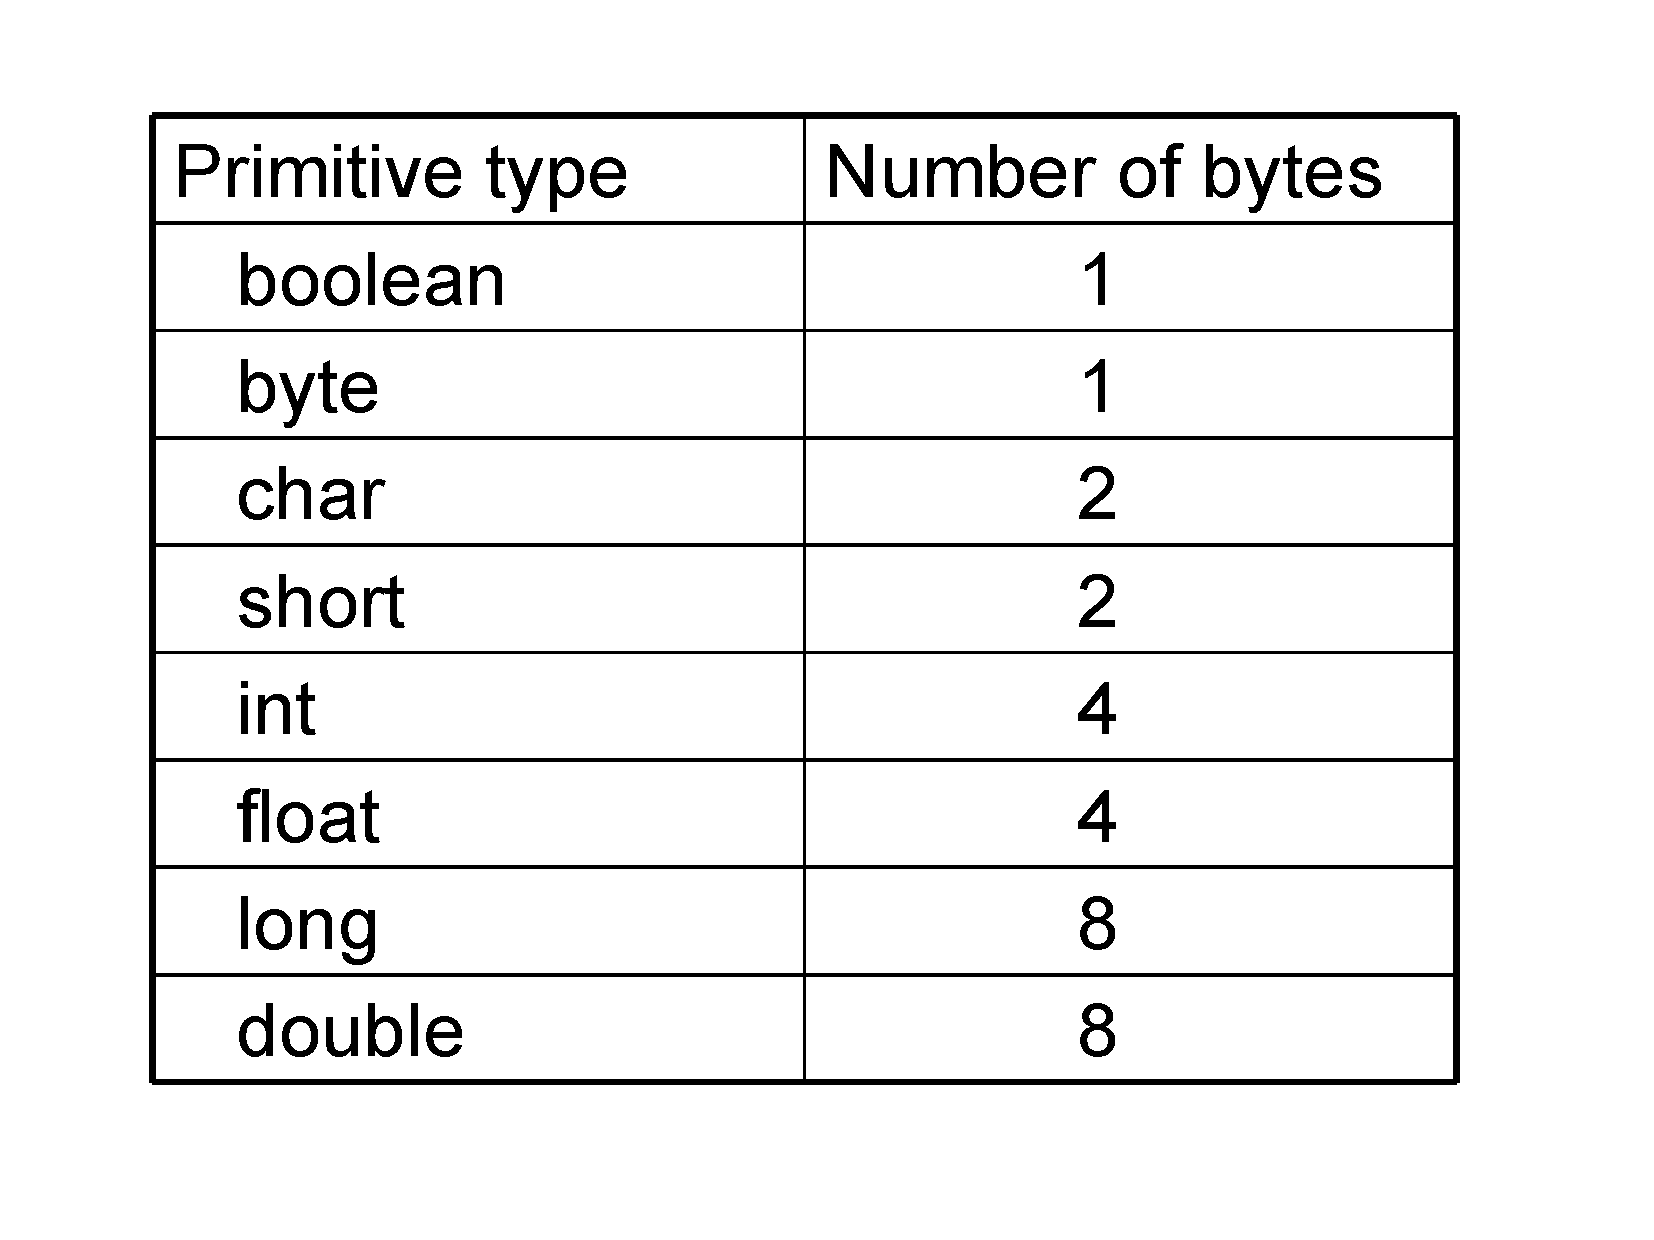
\includegraphics[width=.50\textwidth]{part1/Figures/modelingdatatypes/primitive-byte-sizes.pdf}
\begin{tabular}{lc} \toprule
	Data type & Number of bytes \\ \midrule
	boolean, byte & 1 \\
	char, short & 2 \\
	int, float & 4 \\
	long, double & 8 \\
	reference (32-bit \jre) & 4 \\
	\bottomrule
\end{tabular}
 % 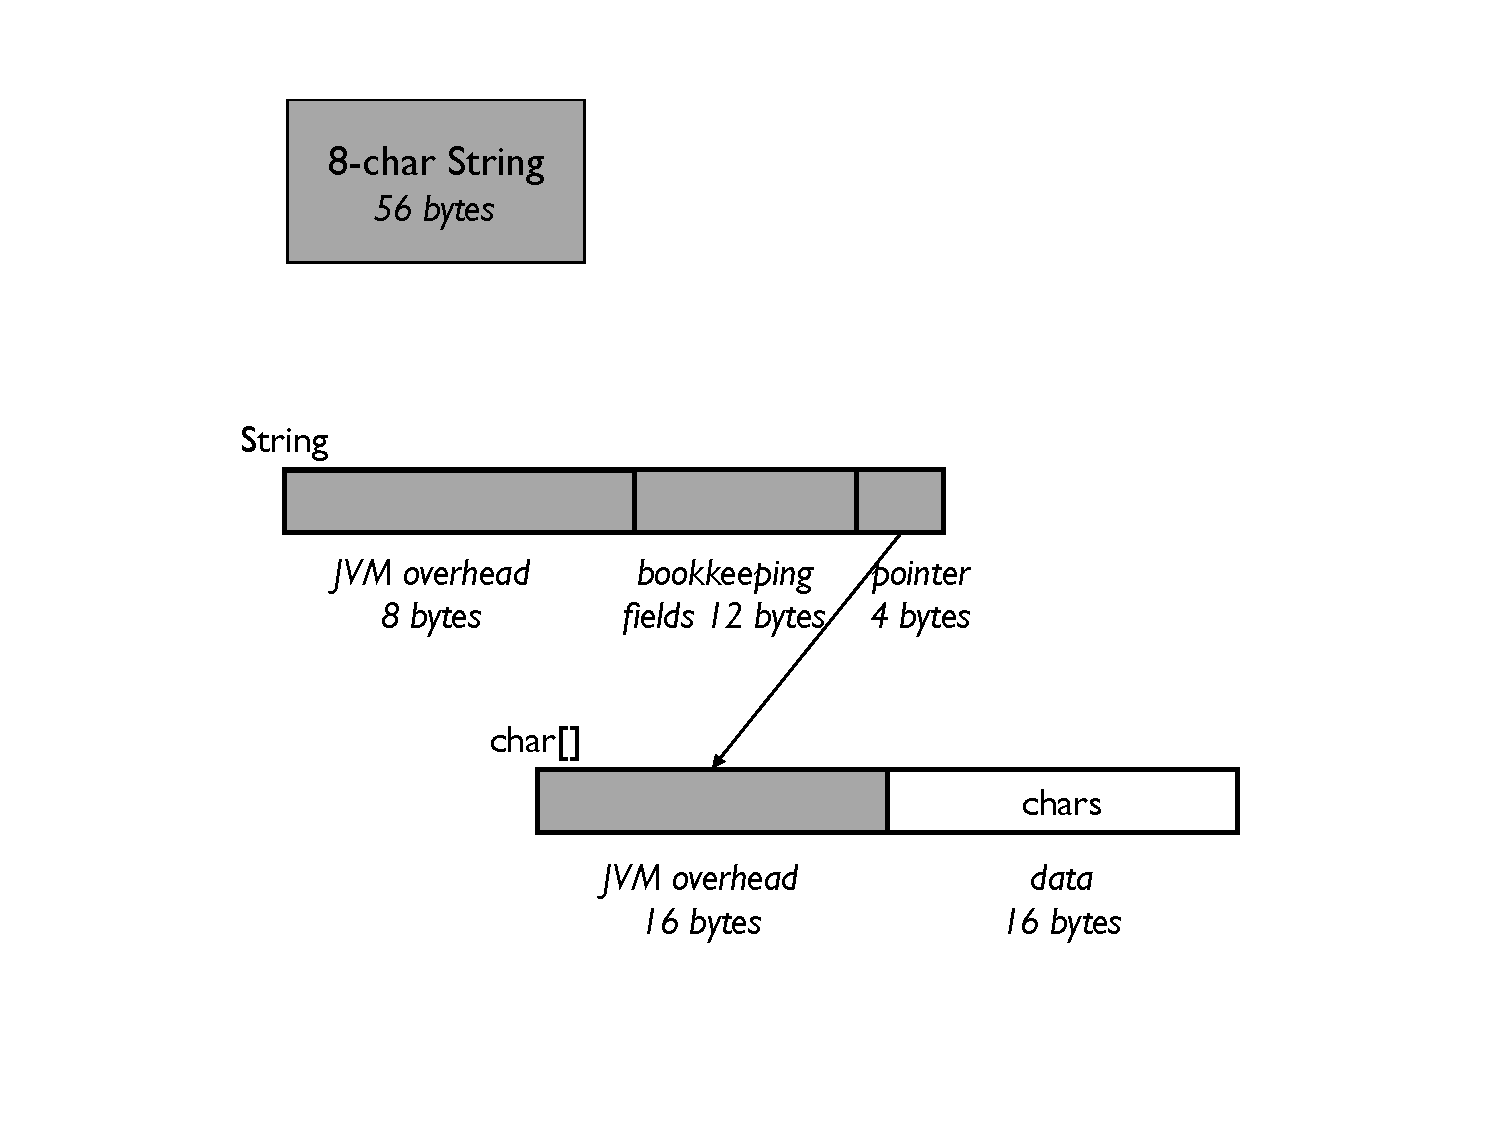
\includegraphics{eight-char-string}
  \caption{The number of bytes needed to store primitive data and reference
  fields.}
  \label{tab:primitive-sizes}
\end{table}

\paragraph{Object-level overhead} Objects are bigger than the sum of their
fields, and their size depends on the specific \jre implementation. The \jre allocates a header with each object that
stores information such as the object's class, an identity hashcode, a monitor
used for locking, and various flags. For array objects, the header has an
additional integer to store the number of array elements. Additionally,  the
\jre requires objects to be aligned on specific address boundaries, for example,
addresses that are multiples of 8. To show how implementations differ,
Table~\ref{tab:object-overhead} gives object header and alignment costs imposed
by two \jres, \oracle \javasix and \ibm \javasix,
both for 32-bit architectures. \footnote{Unless otherwise noted, all of the
numbers throughout the book are based on the \oracle \jre for 32-bit architectures.
Appendix~\ref{chapter:jre-comparison} gives information needed to estimate
sizes in various environments.}
\begin{table}
  \centering
 %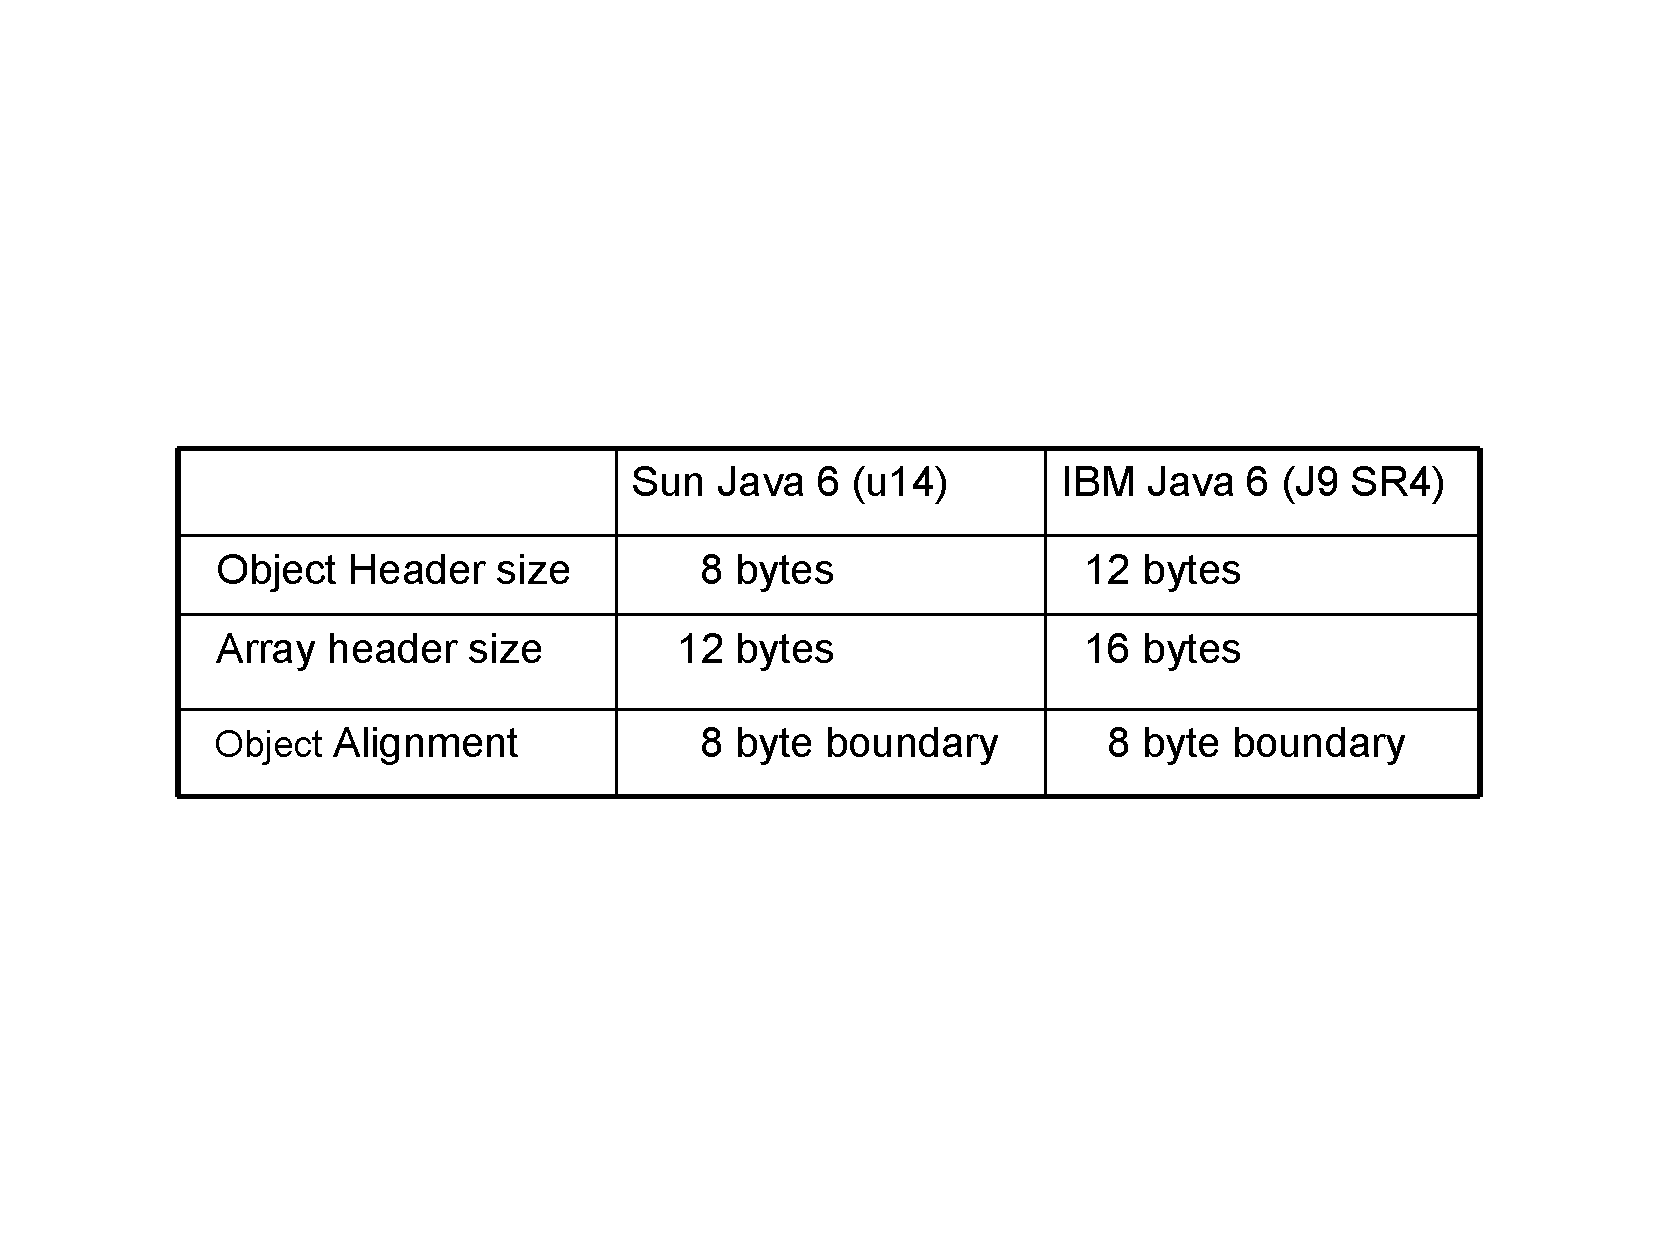
\includegraphics[width=.70\textwidth]{part1/Figures/modelingdatatypes/object-overhead.pdf}
 % 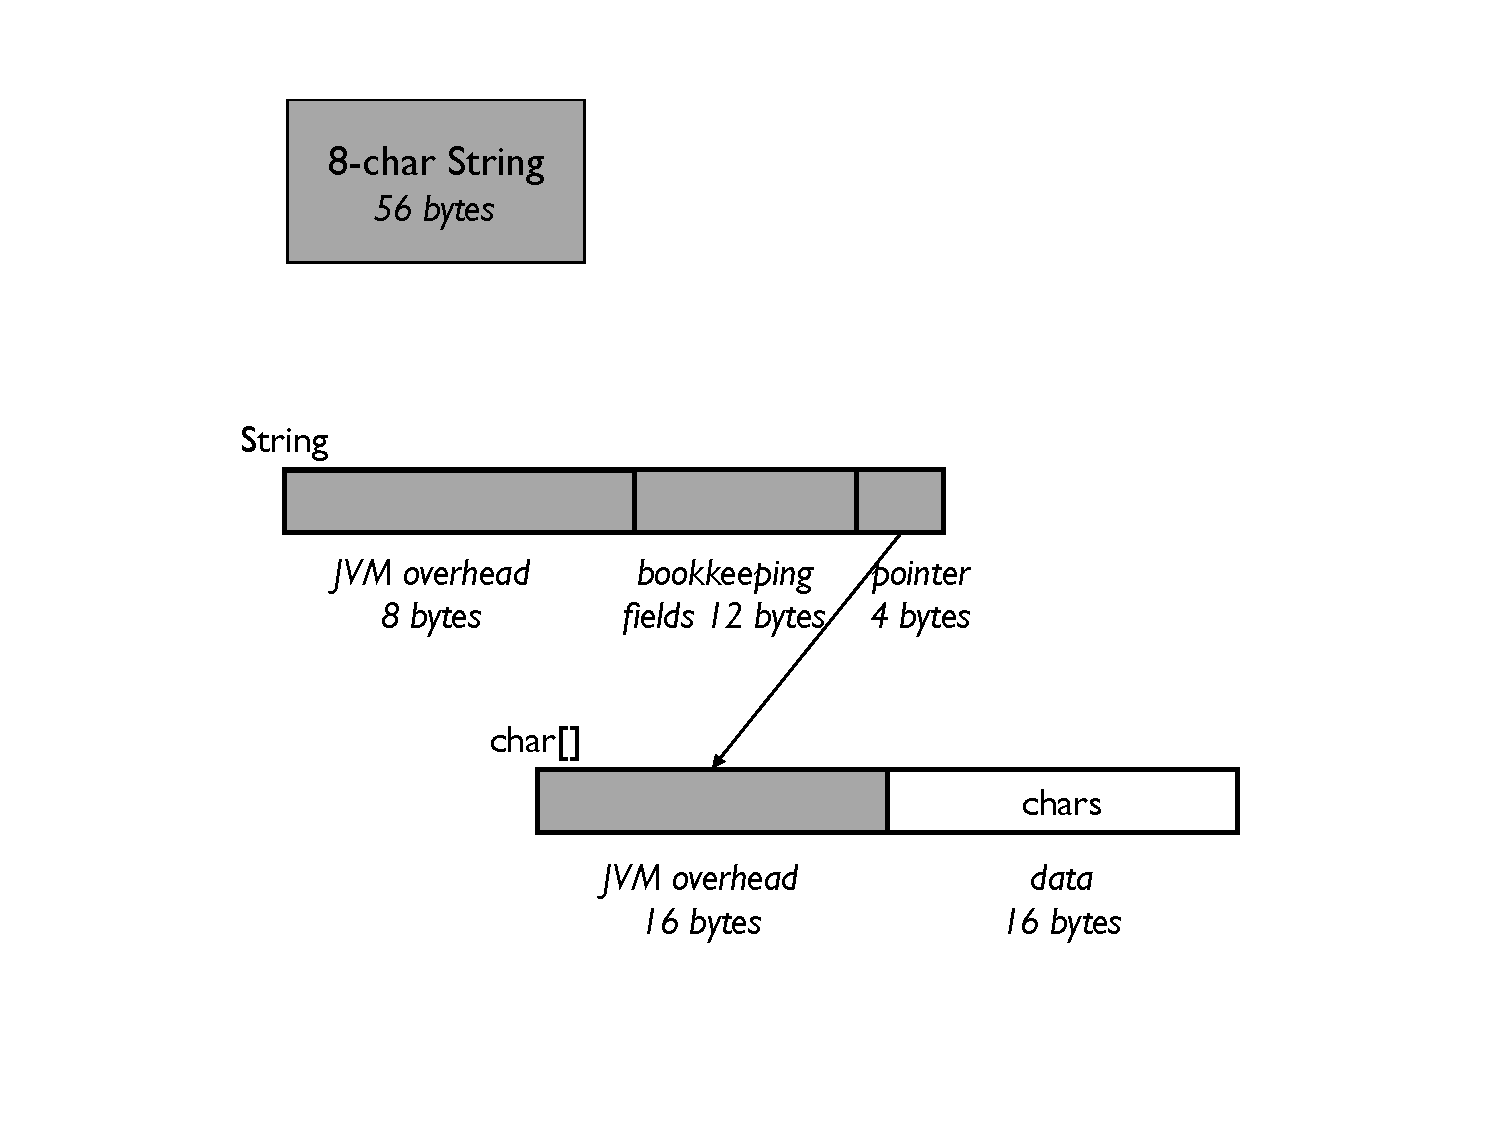
\includegraphics{eight-char-string}
 \begin{tabular}{lll} \toprule
 	& \oracle \javasix & \ibm \javasix \\ \midrule
 	Object header size & 8 bytes & 12 bytes \\
 	Array header size & 12 bytes & 16 bytes \\
 	Object alignment & 8 byte boundary & 8 byte boundary \\
 	Minimum field alignment & 1 byte boundary & 4 byte boundary \\
 	\bottomrule
 \end{tabular}
  \caption{Object overhead used by the \oracle and \ibm \jres for 32-bit architectures.}
  \label{tab:object-overhead}
\end{table} 
   %The \oracle JVM allocates 8 bytes per object header, and the \ibm JVM allocates 12 bytes per header. 
   
The simplest objects are the boxed scalars, which are objects with a single
primitive data type field. Since both of these \jres align objects on
8-byte boundaries and object headers are at least 8 bytes, a boxed scalar takes
at least 16 bytes. Table~\ref{tab:boxed-scalar-sizes} gives the sizes of boxed
scalars.

\begin{table}
  \centering
%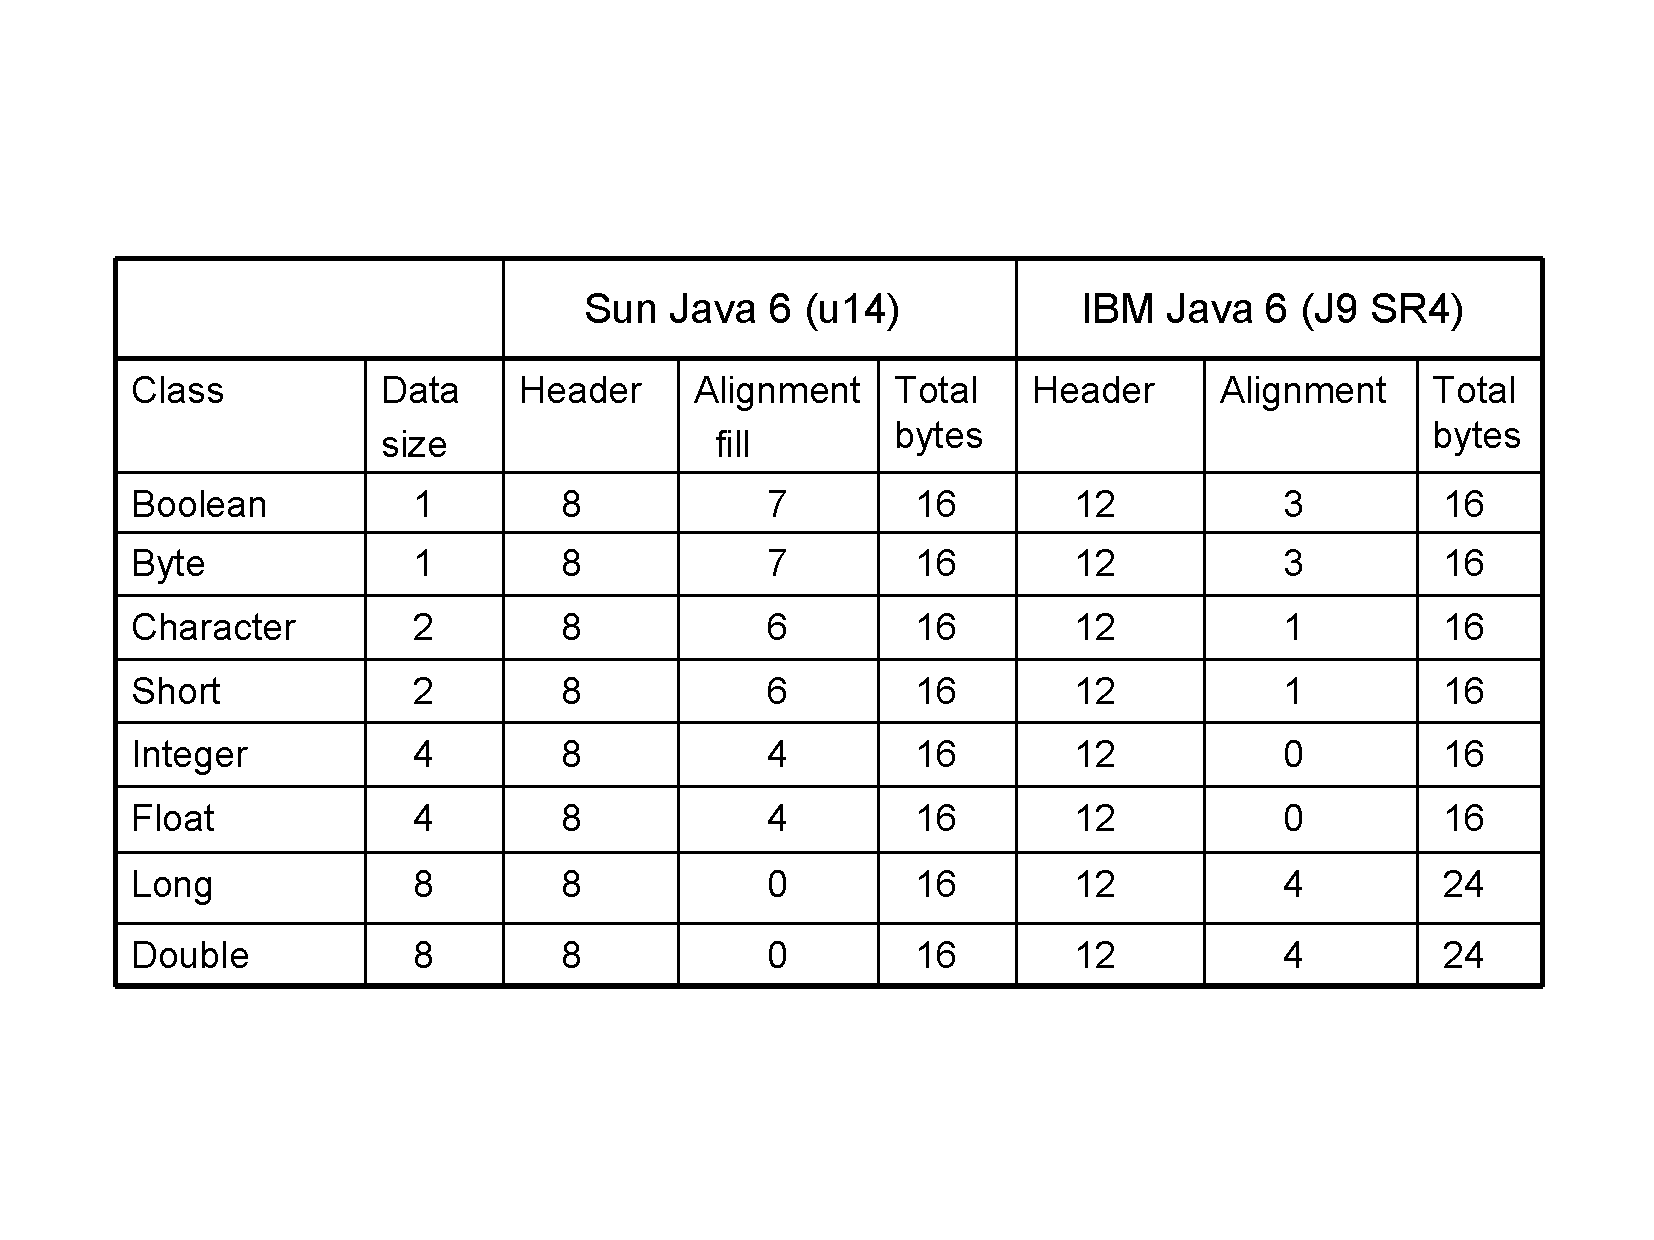
\includegraphics[width=.70\textwidth]{part1/Figures/modelingdatatypes/boxed-scalar-sizes.pdf}
	\begin{tabular}{lccccccc} \toprule
    	& & \multicolumn{3}{c}{\oracle \javasix} & \multicolumn{3}{c}{\ibm
    	\javasix} \\ \cmidrule(r){3-5} \cmidrule(l){6-8}
    	%
    	Class & \shortstack[c]{Data\\size} & Header & \shortstack{Align-\\ment
    	fill} & \shortstack[c]{Total\\bytes} & Header & \shortstack{Align-\\ment
    	fill} & \shortstack[c]{Total\\bytes}
    	\\ \midrule 
    	%
    	{Boolean,} & \multirow{2}{*}{1} & \multirow{2}{*}{8} & \multirow{2}{*}{7} &
    	\multirow{2}{*}{16} & \multirow{2}{*}{12} & \multirow{2}{*}{3} &
    	\multirow{2}{*}{16}
    	\\
    	Byte & \\ \addlinespace
    	%
    	Character, & \multirow{2}{*}{2} & \multirow{2}{*}{8} & \multirow{2}{*}{6}
    	& \multirow{2}{*}{16} & \multirow{2}{*}{12} & \multirow{2}{*}{1} &
    	\multirow{2}{*}{16} \\
    	Short & \\ \addlinespace
    	%
    	Integer, & \multirow{2}{*}{4} & \multirow{2}{*}{8} & \multirow{2}{*}{4} &
    	\multirow{2}{*}{16} & \multirow{2}{*}{12} & \multirow{2}{*}{0} &
    	\multirow{2}{*}{16}
    	\\
    	Float & \\ \addlinespace
    	%
    	Long, & \multirow{2}{*}{8} & \multirow{2}{*}{8} & \multirow{2}{*}{0} &
    	\multirow{2}{*}{16} & \multirow{2}{*}{12} & \multirow{2}{*}{4} &
    	\multirow{2}{*}{24} \\
    	Double & \\
		\bottomrule
	\end{tabular}
  \caption{The sizes of boxed scalar objects, in bytes, for 32-bit
  architectures.}
  \label{tab:boxed-scalar-sizes}
\end{table}
 
\paragraph{Field-level overhead} Estimating the size of an object with more
than one field is a bit more complicated, since the hardware imposes additional
alignment requirements on specific data types. For example, integer fields are
usually aligned on 4 byte boundaries. This field alignment potentially introduces more padding.

%\begin{example}{Simple Employee Class.}
For example, consider a class \class{SimpleEmployee}, which has all primitive fields.
The comments show the number of bytes needed to store the primitive data.

\begin{shortlisting}
class SimpleEmployee {
    int id;               // 4 bytes
    int hoursPerWeek;     // 4 bytes       
    boolean exempt;       // 1 byte          
    double salary;        // 8 bytes          
    char jobCode;         // 2 bytes           
    int yearsOfService;   // 4 bytes      	
}
\end{shortlisting}
%\end{example}

If the fields are laid out one after the other with no fill, then the
field \class{salary} would have to begin on a 5-byte boundary, which is not allowed for
\class{doubles}. To avoid adding 3 more bytes of padding, the \jre could rearrange the fields
to take up the smallest amount of space. In fact, the \oracle \jre does a good job rearranging and
packing fields, and the \ibm \jre does not. This means that field sizes depend on the specific \jre also. 

Using the \oracle \jre, you can assume each field is the size of its primitive data type because the fields are packed. The size of a
\class{SimpleEmployee} object is 32 bytes:

\begin{shortlisting}               
8 + (4+4+1+8+2+4) = 31 bytes, rounds up to 32 bytes
\end{shortlisting} 

In contrast, using the \ibm \jre, all fields in non-array objects are either 4
or 8 bytes. Here is the \class{SimpleEmployee} class with field sizes adjusted
accordingly.
\begin{shortlisting} 
class SimpleEmployee {
    int id;                  // 4 bytes
    int hoursPerWeek;        // 4 bytes
    boolean exempt;          // 4 byte
    double salary;           // 8 bytes
    char jobCode;            // 4 bytes
    int yearsOfService;      // 4 bytes
}
\end{shortlisting}
The size of a \class{SimpleEmployee} is 40 bytes:
\begin{shortlisting}
12 + (4+4+4+8+4+4) = 40 bytes, with no object alignment needed
\end{shortlisting}

\paragraph{Arrays} For arrays, the data is always packed with no spaces. For
example, here is a formula that estimates the size of an array of 100 \code{chars}:
\begin{shortlisting}
header + 100*2, round up to a multiple of the object alignment
\end{shortlisting}

\callout{callout:minimum-size-estimation-rule}{Estimating Object Sizes}{
\index{Estimating Object Size}
The size of an object can be estimated as follows:
\begin{enumerate}
\item Add together the sizes of all of the fields and the object header. Fields include those in the object's class and all of its superclasses.
\item Round up the result to the next multiple of the object alignment.
\end{enumerate}
The object header size and alignment depend on the \jre.
Field sizes also depend on the \jre. For example, the \jre may pack fields to obtain the minimum
possible size, or align fields on word boundaries. Array data is always packed. }

For objects with only a small amount of primitive data, the overhead is relatively high. 
But as the amount of primitive data increases, the bloat factor decreases. 
The overhead cost consists of a fixed object header cost and a bounded
object alignment cost, which become less significant when there is more data. 
For example, for the \oracle \jre, the bloat factors for the boxed scalars range from 94\%
for a \class{Boolean} down to 50\% for a
\class{Double}.  The bloat factor for a \class{SimpleEmployee} is 28\%.  The
bloat factor for an array of 100 \code{chars} is insignificant.  
An exception to this rule is when objects
have a lot of fields, such as \code{booleans}, that carry very little data, on
a \jre that doesn't pack fields tightly.
These objects will have a high bloat factor. In that case, the more fields, the
more overhead.

\section{The Cost of Delegation}
\index{Delegation}

The \class{SimpleEmployee} class is not very realistic, since it has only
primitive fields. Usually, a class has some fields that are objects. In Java,
this kind of field is implemented using
\textit{delegation}, that is, by storing a reference to another object. 
Some of the most common field types are modeled this way, requiring one or more
separate objects. Table~\ref{tab:common-delegated-field-types} shows the space
needs of the most common ones.


\begin{table}[htbp]
  \centering
%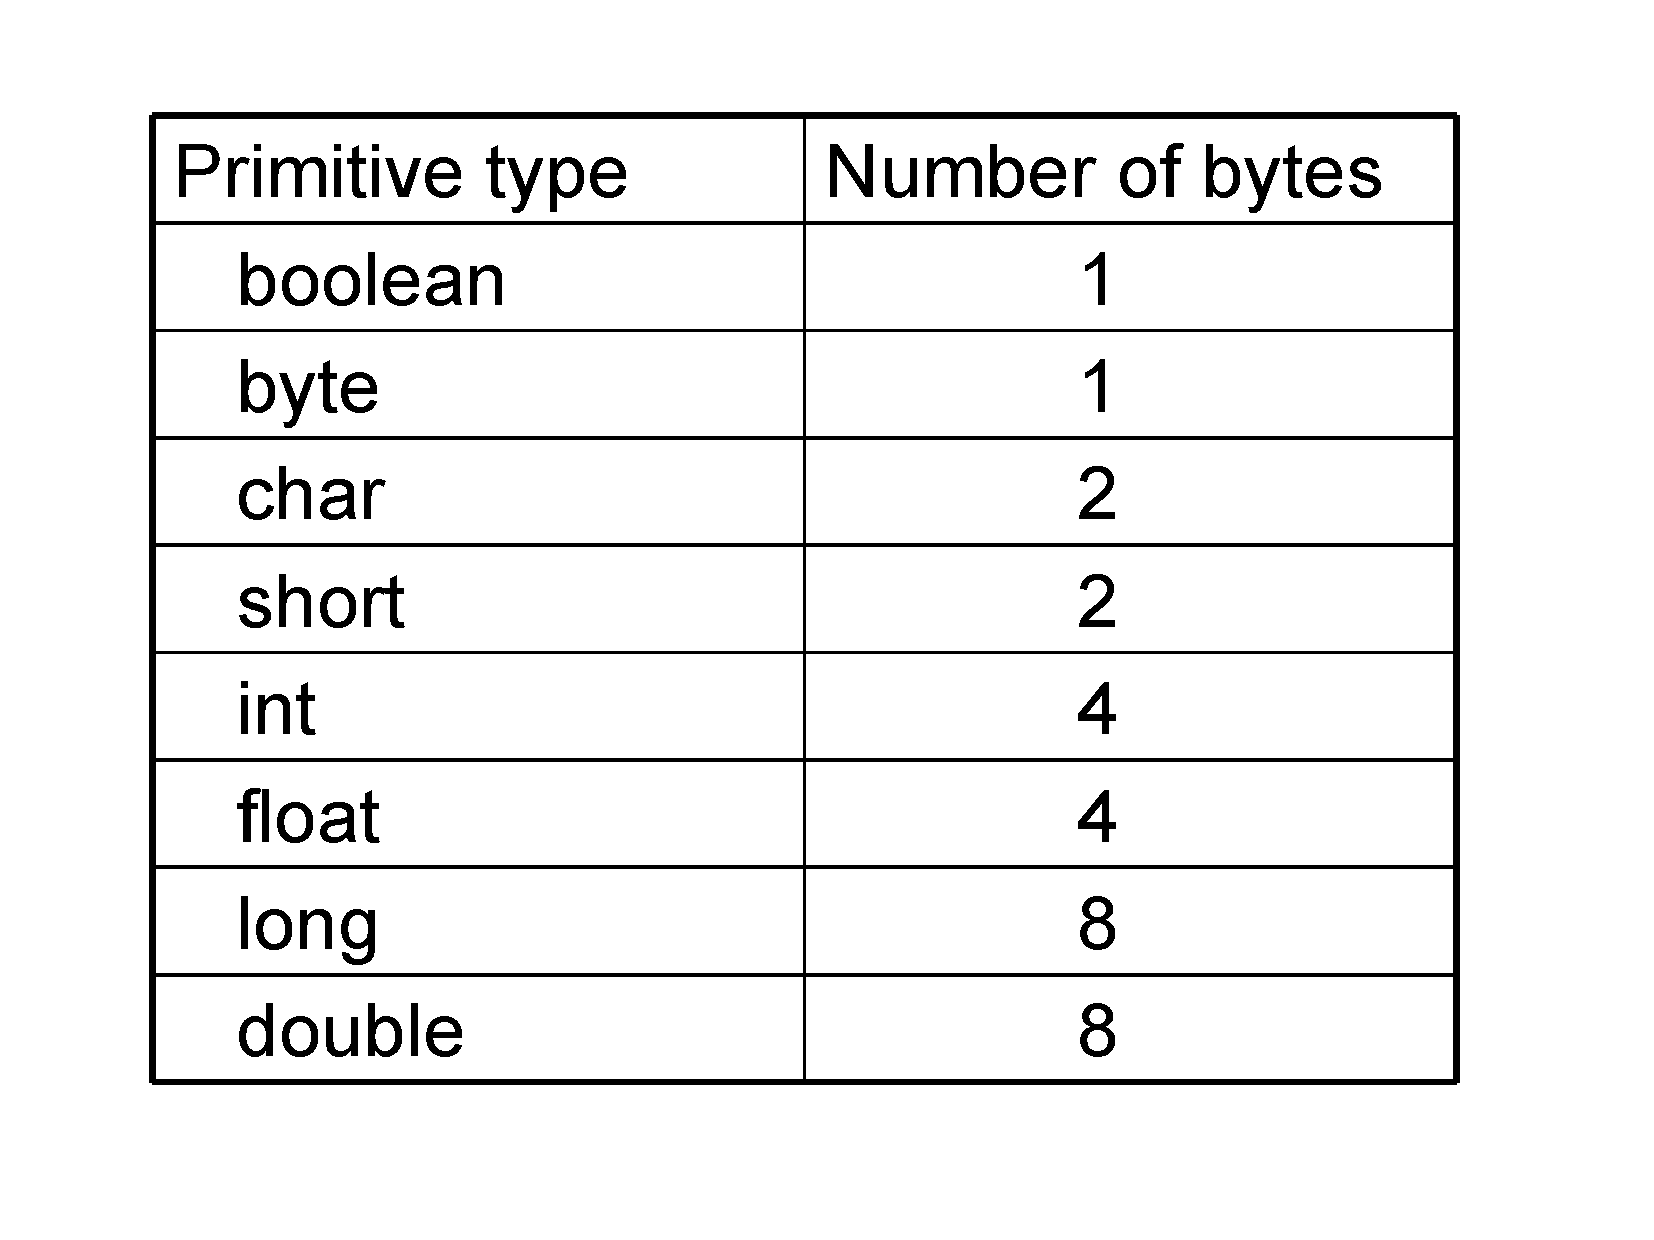
\includegraphics[width=.50\textwidth]{part1/Figures/modelingdatatypes/primitive-byte-sizes.pdf}
\begin{tabular}{lcc} \toprule
	Class & Number of objects & Size in bytes \\ \midrule
	String (8-character) & 2 & 56 \\
	Date & usually 1, up to 4 & 24, when 1 object \\
	BigDecimal & usually 1, up to 5 & 32, when 1 object \\
	Enum & 0, uses a shared object & 0 \\
	\bottomrule
\end{tabular}
 % 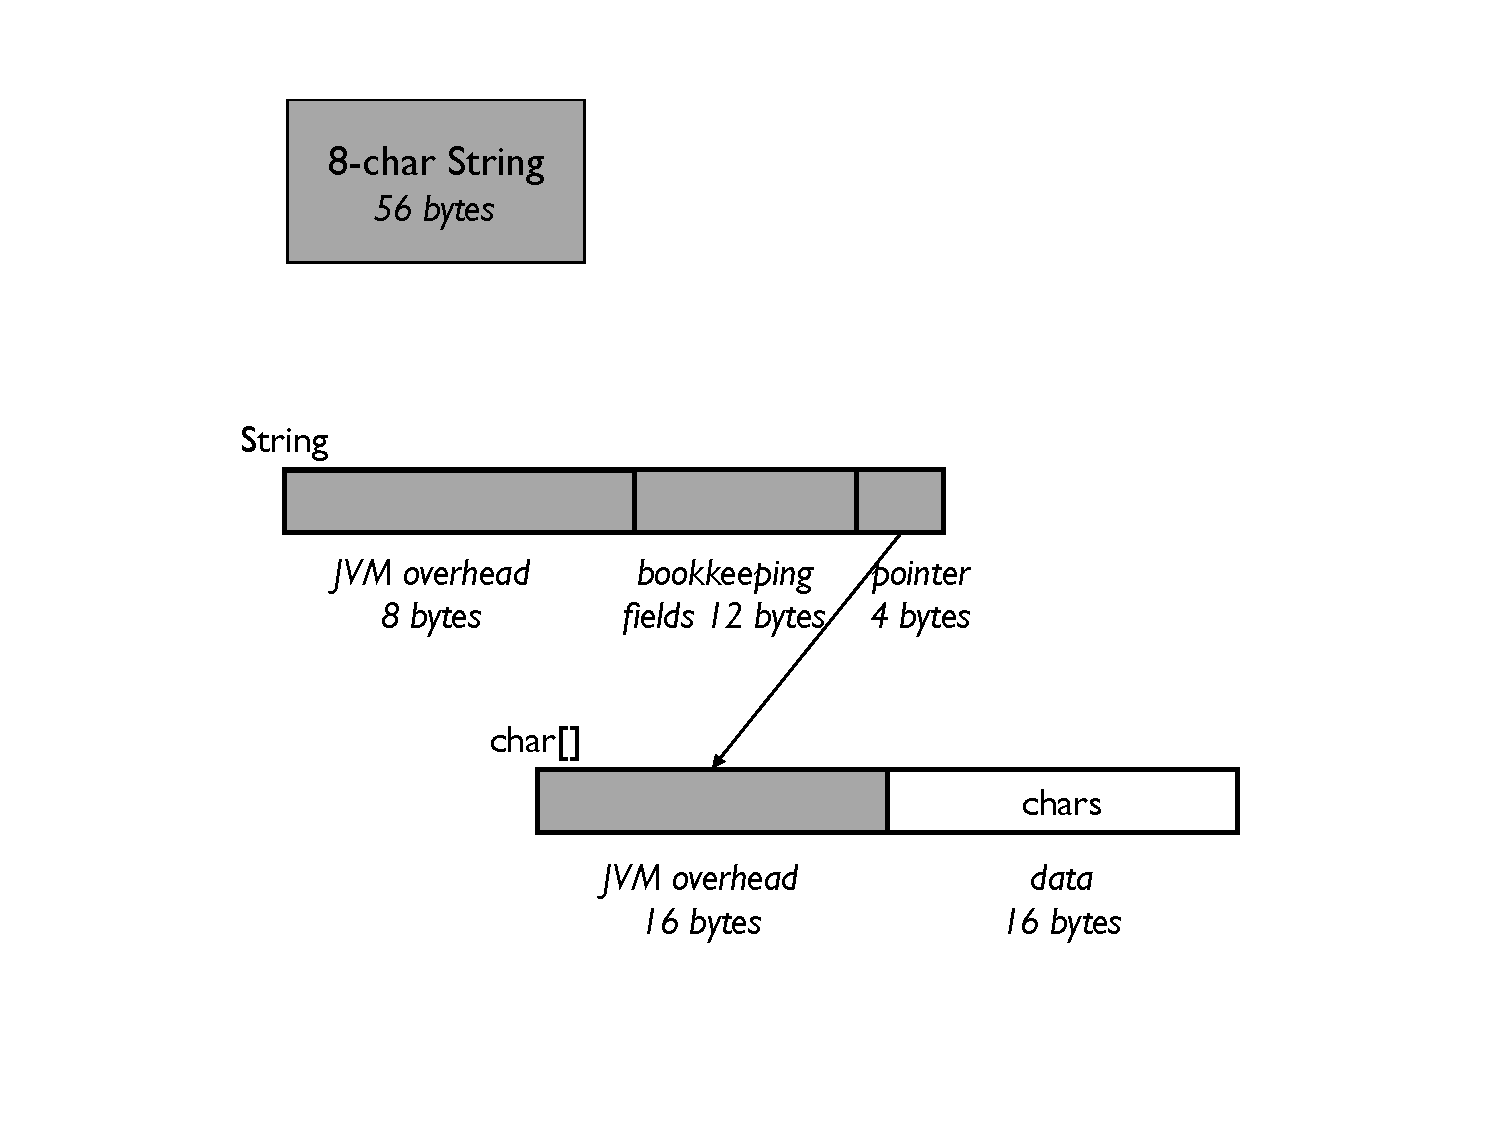
\includegraphics{eight-char-string}
  \caption{Memory requirements for some common field types that require one
  or more separate objects. Sizes do not include a referring pointer.
  }
  \label{tab:common-delegated-field-types}
\end{table}


%\begin{example}{Employee class with delegation}
Here is a more realistic employee class with several reference fields. An
employee now has a name, which is a \class{String}, instead of an integer id. It
also has a start date, which is a \class{Date}. The type of \class{salary} has
been changed from \code{double} to \class{BigDecimal}. \class{BigDecimal} avoids potential roundoff errors.
\begin{shortlisting} 
class Employee {
    String name;                // 4 bytes
    int hoursPerWeek;           // 4 bytes
    BigDecimal salary;          // 4 bytes
    Date startDate;             // 4 bytes
    boolean exempt;             // 1 byte
    char jobCode;               // 2 bytes
    int yearsOfService;         // 4 bytes
}
\end{shortlisting}

On 32-bit architectures, a pointer is 4 bytes. 
You can calculate the size of any object as described in
Section~\ref{sec:CostOfObjects}.
Assuming the \oracle \jre, the size of an \c{Employee} object is 32 bytes:
\begin{shortlisting}
8 + (4+4+4+4+1+2+4) = 31, rounds up to 32 bytes
\end{shortlisting}
%\end{example}

While an instance of the \class{Employee} class is a single 32
byte object, an entire employee, including name, salary, and start date
consists of at least five objects. Two of these objects
are used to store the name. (Recall from Section~\ref{sec:bloat-def} that a string is represented by a
wrapper \class{String} object and a \class{char} array.) \class{BigDecimal}
usually requires 1 object but can take up to 5 depending on the usage.
The memory layout for a specific employee ``John Doe" is shown in Figure~\ref{fig:employee-status}.
 \begin{figure}
  \centering
 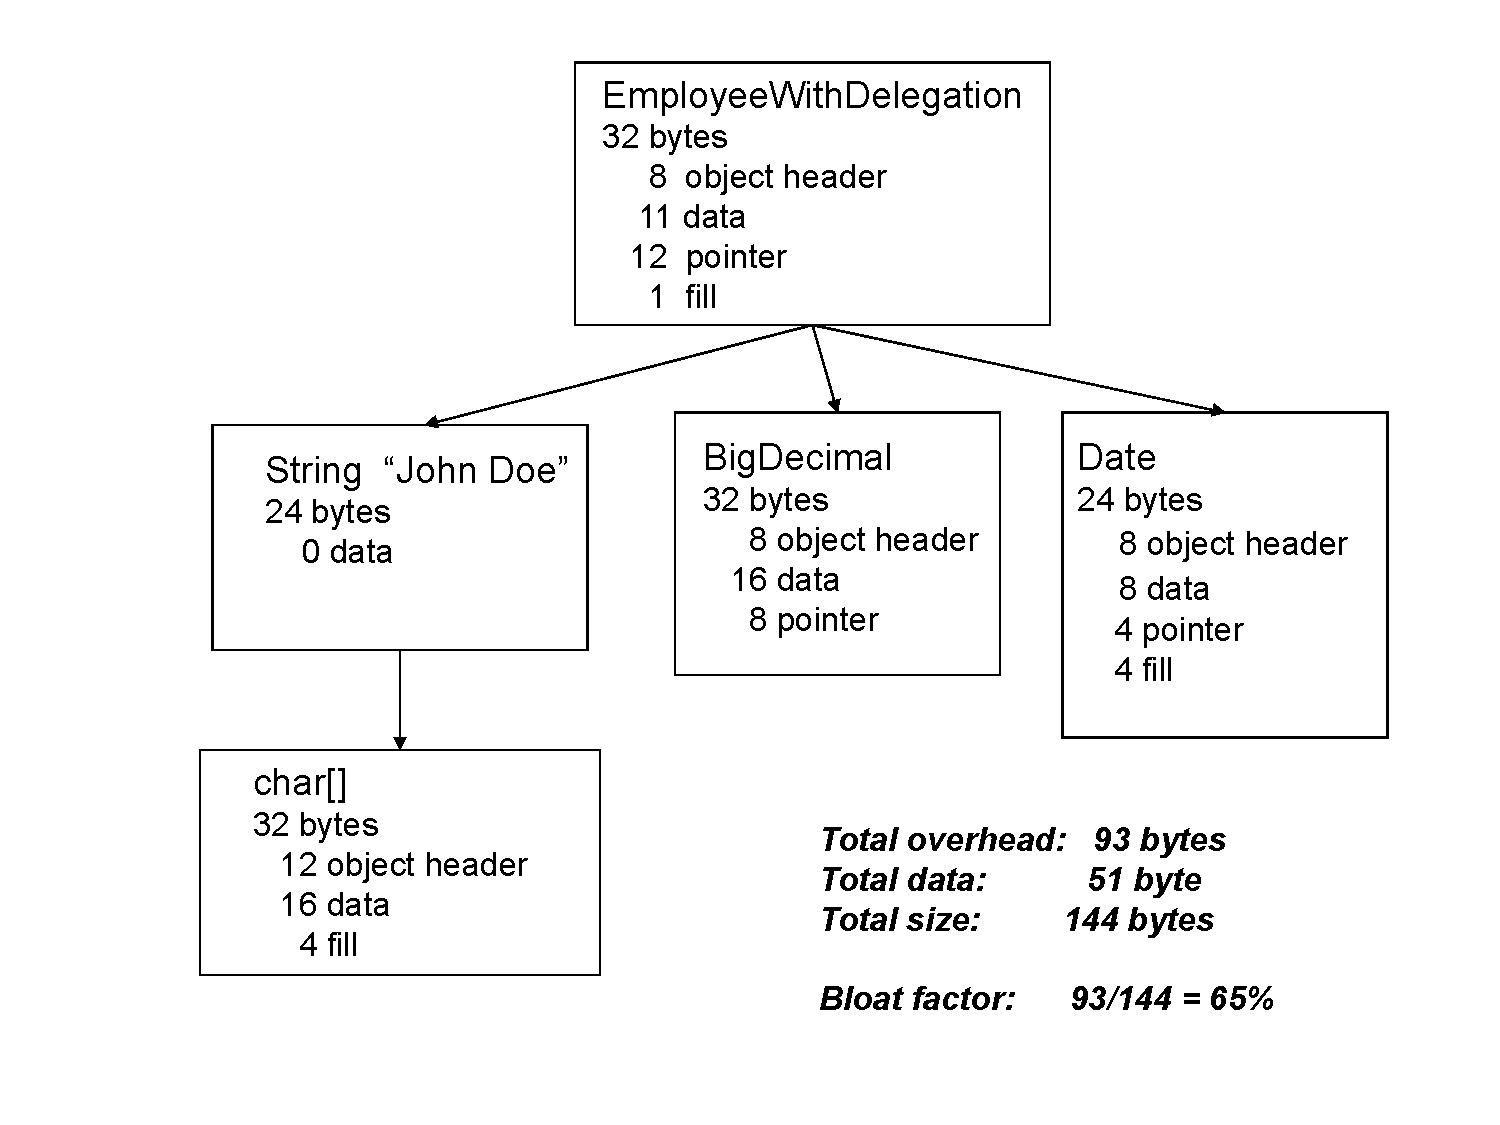
\includegraphics[width=.80\textwidth]{part1/Figures/modelingdatatypes/employee-status.pdf}
 % 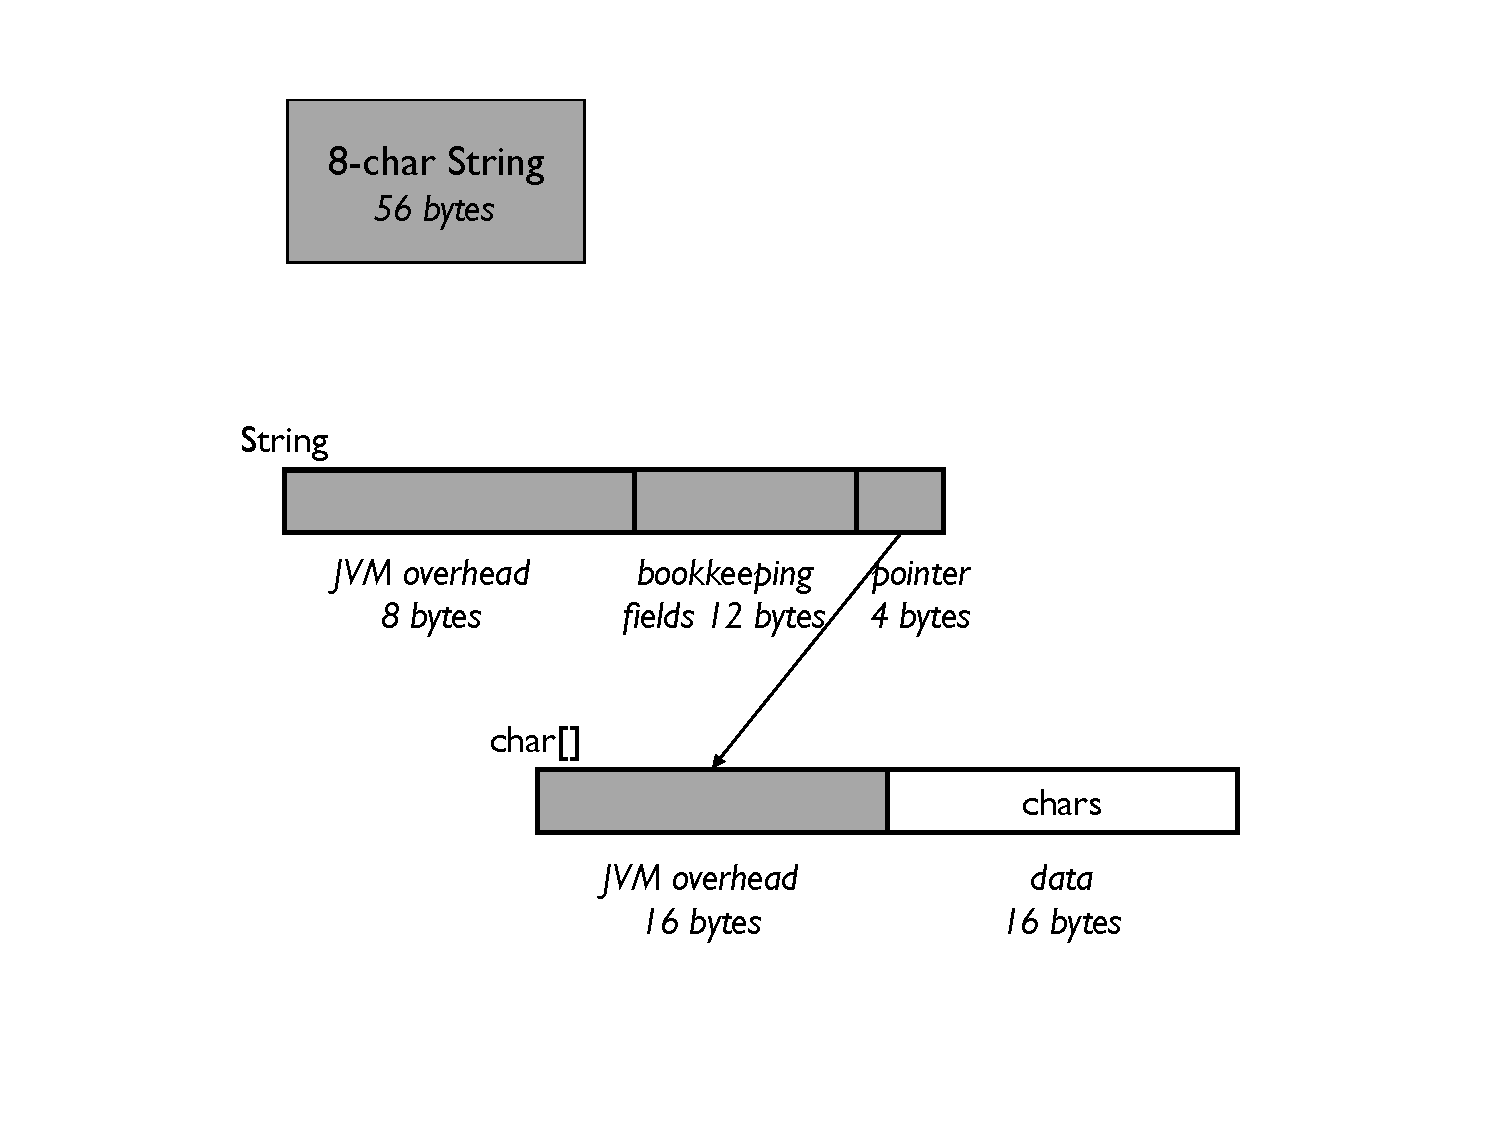
\includegraphics{eight-char-string}
  \caption{The memory layout for an employee, with some field data
  delegated to additional objects.}
  \label{fig:employee-status}
\end{figure}



A comparison of an \class{Employee} object with a
\class{SimpleEmployee} object from Section~\ref{sec:CostOfObjects} shows that
the size has increased from 32 to 144 bytes, and the bloat factor has increased
from 28\% to 65\%.
There is more information stored in the new version, so it is no surprise that it is bigger. The increase
in the bloat factor is more significant. Delegation increases memory bloat. Delegation introduces additional
object headers, and a pointer for each delegated object, including empty
pointer slots for uninitialized object fields. In this example, the
4 new object headers and 7 pointer slots add up to 60 bytes, or
42\% of the total memory of an \class{Employee} record. Delegation may also
force additional alignment costs, since each new delegated object has to be aligned
to an 8-byte boundary.

\paragraph{Java's Delegation Bias} In the spirit of keeping things simple,
Java does not allow you to embed one object in another. 
% to build a single object out of other objects.
You also cannot nest an array inside an object, or store objects directly in an
array. You can only point from one object to another. Even the basic
data type \class{String} consists of two objects. Single inheritance is the only language feature
that can be used instead of delegation to compose two types, but single
inheritance has limited flexibility. This means that delegation is pervasive
in Java programs. In contrast, C++ gives you many options: 
you can embed one type within another, overlay types using unions, 
employ subclasses with single or multiple inheritance, and point from
one type to another.

% and it is difficult to avoid a high level of delegation overhead.
\callout{callout:estimating-string-cost}{Calculating the Cost of a
\code{String}}{
\index{Estimating String Cost}
The size of a \code{String} can be computed by adding:
\begin{itemize}
\item The size of the \code{String} wrapper = 24 bytes
\item The size of the \code{char[]} = 12 bytes + 2 * number of characters,
then round up to a multiple of 8
\end{itemize}
This is for the \oracle \jre on the 32-bit architecture.}


Because of the design of Java, there is a basic delegation cost that is hard to eliminate.
This is the cost of object-oriented programming in Java. While it is hard to avoid this basic
delegation cost, it is important not to make things a lot worse, as discussed in the next section. 

\section{Fine-Grained Data Models}
\label{fine-grained-data-models}

The software engineering culture tends to promote delegation, and for good reasons. 
Delegation provides a loose coupling of objects, making refactoring and reuse easier. 
Replacing inheritance by delegation is often recommended, especially if the base class
has extra fields and methods that the subclass does not need. In languages with single inheritance,
once you have used up your inheritance slot, it becomes hard to refactor your code. Therefore,
delegation can be more flexible than inheritance for implementing polymorphism. However, overly fine-grained
data models can be expensive both in execution time and memory space. 

There is no simple rule that can always be applied to decide when to use delegation. Each situation has to be evaluated
in context, and there may be tradeoffs among different goals. To make an informed decision, it is important to know what
the costs are.

%\begin{example}{Employee emergency contact} 
\paragraph{Example} Suppose an emergency contact is needed for each employee.
An emergency contact is a person along with a preferred method to reach her. 
The preferred method can be email, cell phone, work phone, or home phone. All contact information for
the emergency contact person must be stored, just in case the preferred method does not work in an actual emergency. 
%\end{example}
Here are class definitions for an emergency contact, written in a highly delegated style that is not uncommon in real applications. 

\begin{shortlisting} 
class EmployeeWithEmergencyContact {
    ...
    EmergencyContact contact;
}
			
class EmergencyContact {
    ContactPerson contact;
    ContactMethod preferredMethod;
}
			
class ContactPerson {
    String name;
    String relation;
    EmailAddress email;
    PhoneNumber phone;
    PhoneNumber cell;
    PhoneNumber work;
}
			
abstract class ContactMethod {
}
			
class PhoneNumber extends ContactMethod {
    byte[] phone;
}
			
class EmailAddress extends ContactMethod {
    String address;
}
\end{shortlisting}
 \begin{figure}
  \centering
 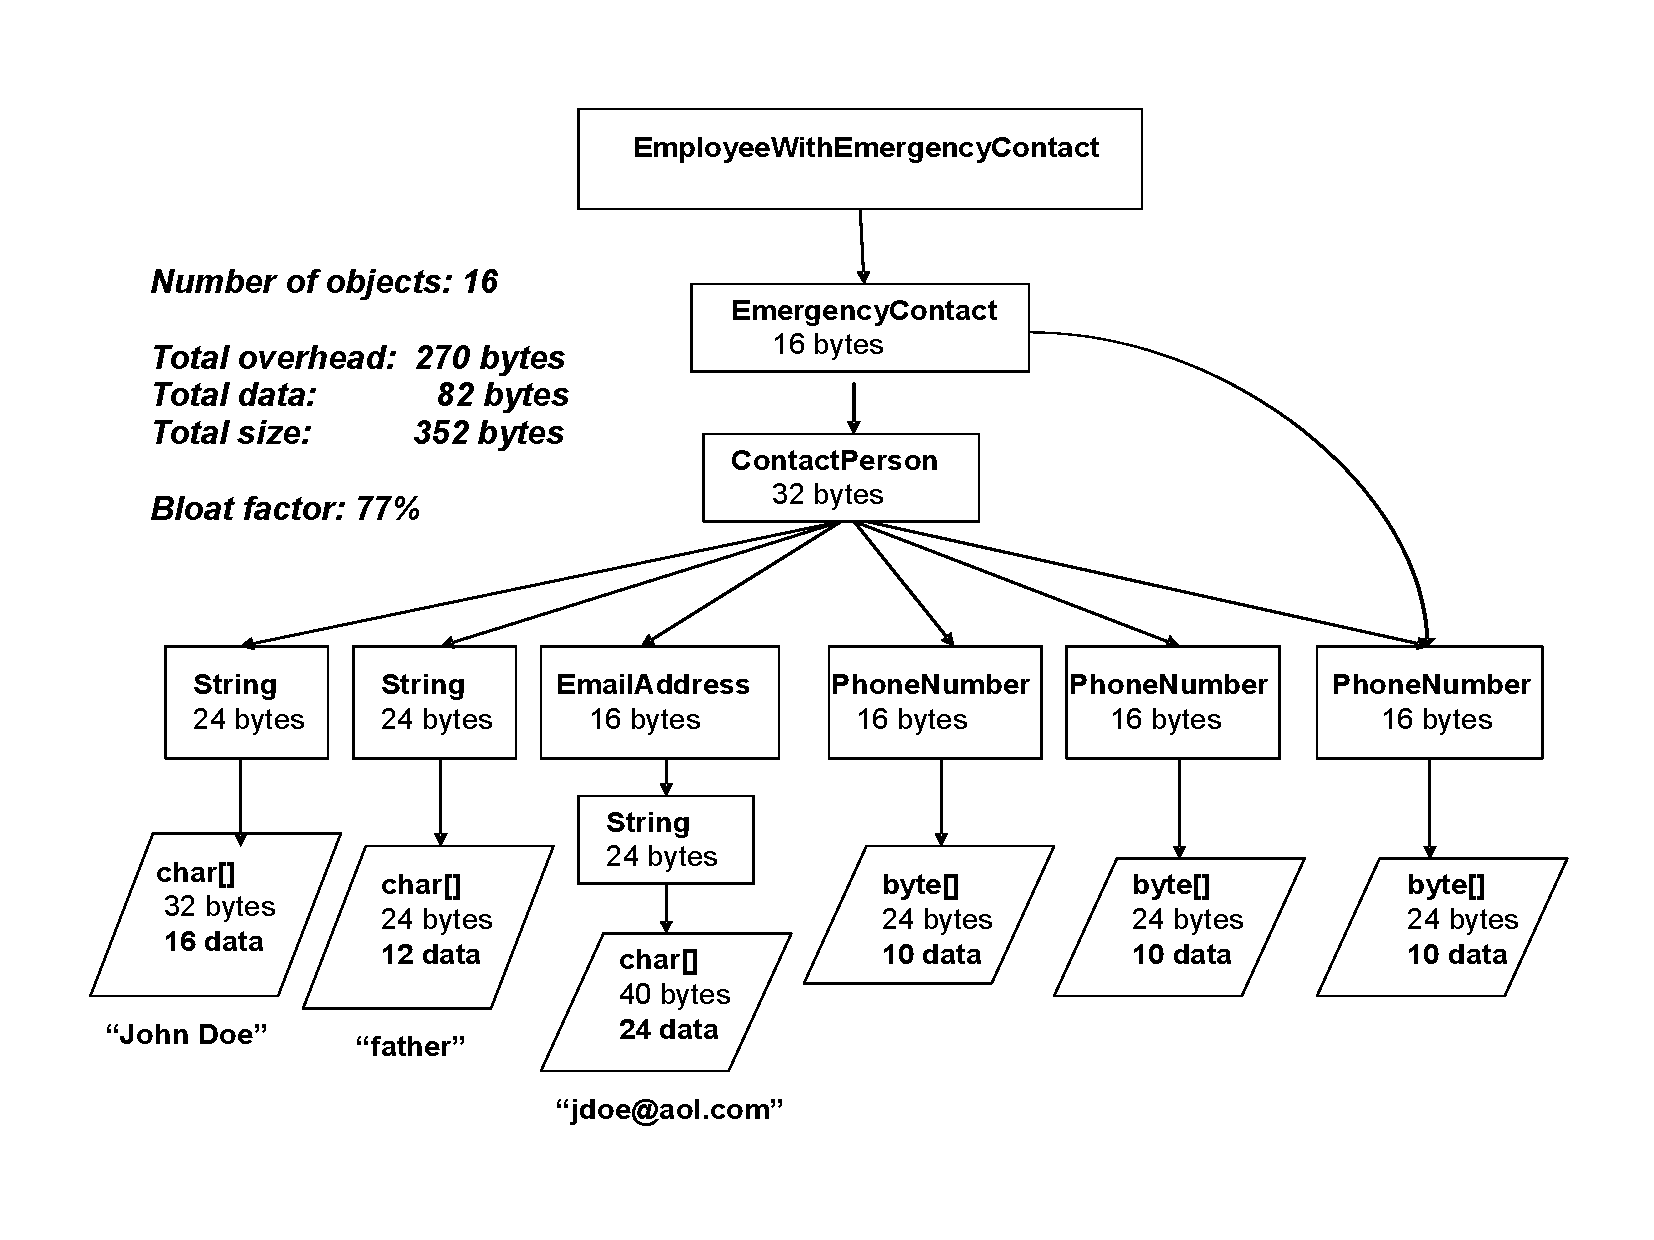
\includegraphics[width=\textwidth]{part1/Figures/modelingdatatypes/employee-status-fine-grained.pdf}
 % 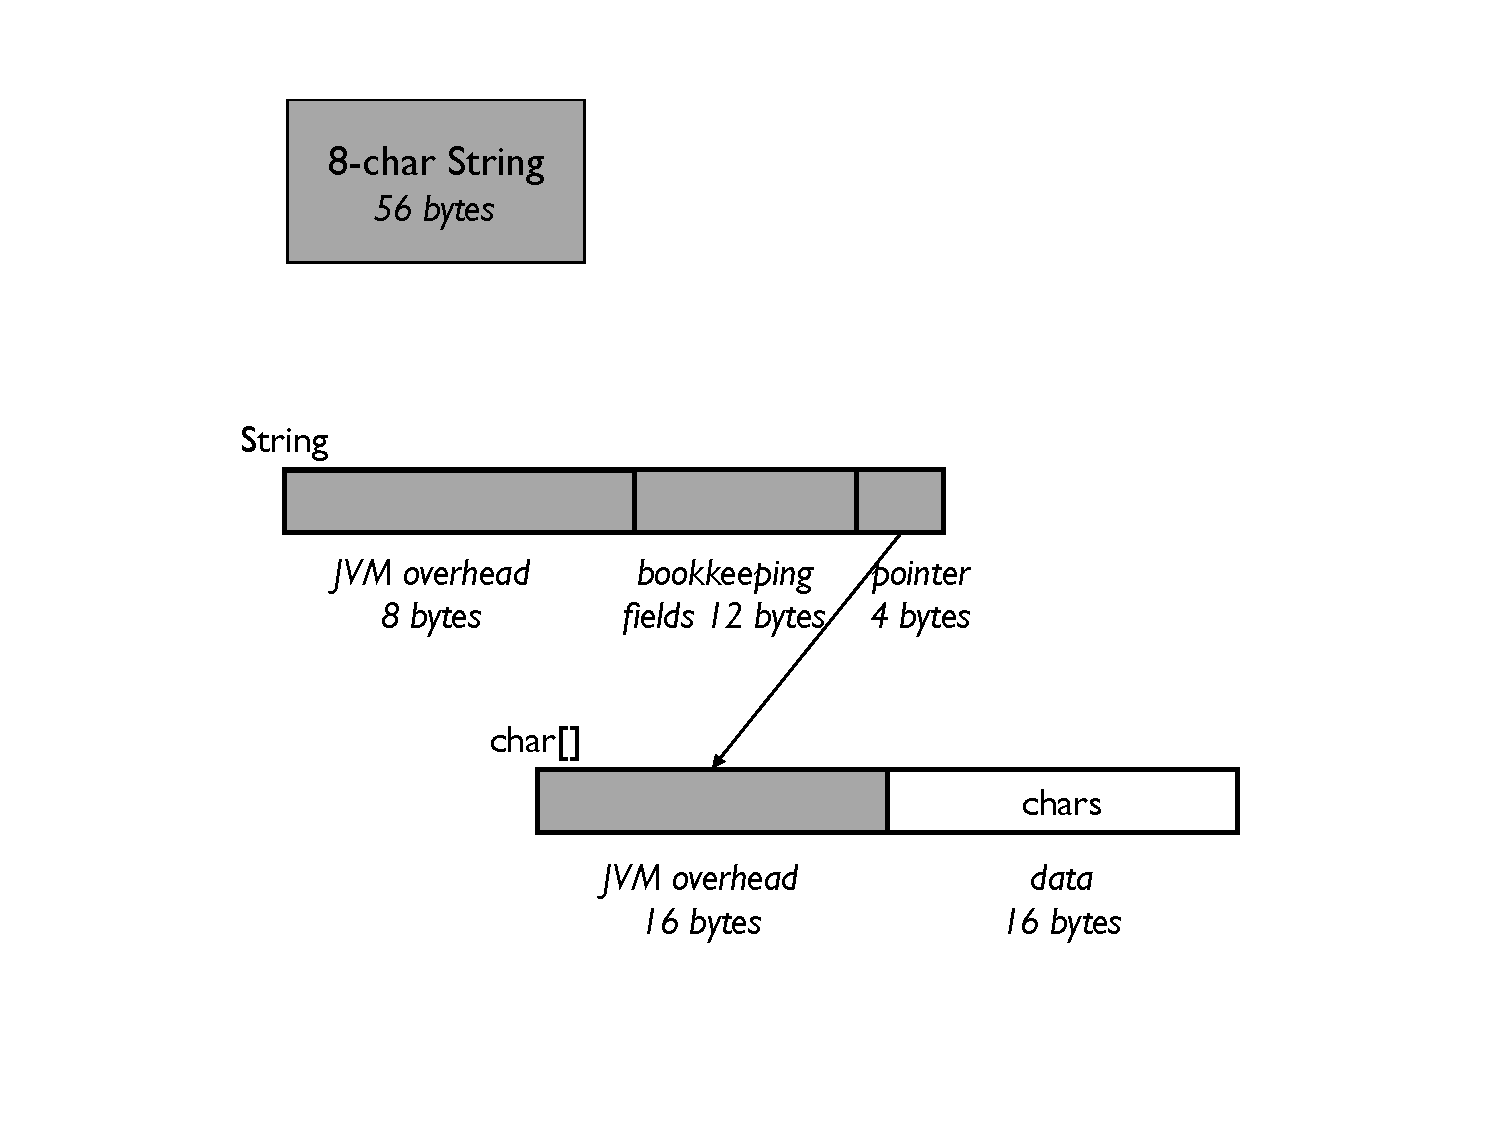
\includegraphics{eight-char-string}
  \caption{The memory layout for an employee with an emergency contact, using
  a fine-grained design.}
  \label{fig:employee-status-fine-grained}
\end{figure}
The memory layout for a sample employee is shown in Figure~\ref{fig:employee-status-fine-grained}. There
are 15 objects used to store emergency contact information, with a bloat factor of 77\%, which seems excessive.
The objects are all small, containing only one or two meaningful fields each,
which is a symptom of an overly fine-grained
data model. Also, all of the data is at the bottom of object chains, 4 to 5 objects long. Refactoring
can flatten this structure somewhat.

\paragraph{Example, optimized} One object that looks superfluous is
\class{EmergencyContact}, which encapsulates the contact person and the
preferred contact method. Removing this delegation involves moving the fields
of \class{EmergencyContact} into other classes, and eliminating the \class{EmergencyContact} class.
Here are the refactored classes:

\begin{nospanshortlisting}
class EmployeeWithEmergencyContact {
    ...
    ContactPerson contact;
}
			
class ContactPerson {
    String name;
    String relation;
    EmailAddress email;
    PhoneNumber phone;
    PhoneNumber cell;
    PhoneNumber work;
    ContactMethod preferredMethod;
}
\end{nospanshortlisting}

This change eliminates an object from
Figure~\ref{fig:employee-status-fine-grained}, but it only recovers 8 bytes,
since a 16 byte object is removed and \class{ContactPerson} is 8 bytes bigger.
You can save considerably more space by inlining the four \class{ContactMethod}
classes into the \class{ContactPerson} class, which removes 64 bytes of
overhead. In a system with many instances of
employees stored in memory, this reduction is significant. In order to make this change,
the preferred contact method must be encoded somehow in \class{ContactPerson}.  A simple way to
achieve this is to use an enumerated type field, which has the same size as a
reference field, to discriminate among the different contact methods:

\begin{shortlisting} 
enum PreferredContactMethod {
    EMAIL, HOME_PHONE, CELL_PHONE, WORK_PHONE;
}
      
class ContactPerson {
    PreferredContactMethod preferredMethod;
    String name;
    String relation;
    String email;
    byte[] cellPhone;
    byte[] homePhone;
    byte[] workPhone;
}		
\end{shortlisting}


Figure~\ref{fig:refactored-fine-grain} shows the memory layout after these changes. Both the size
and the bloat factor have been reduced.
 \begin{figure}[htbp]
  \centering
 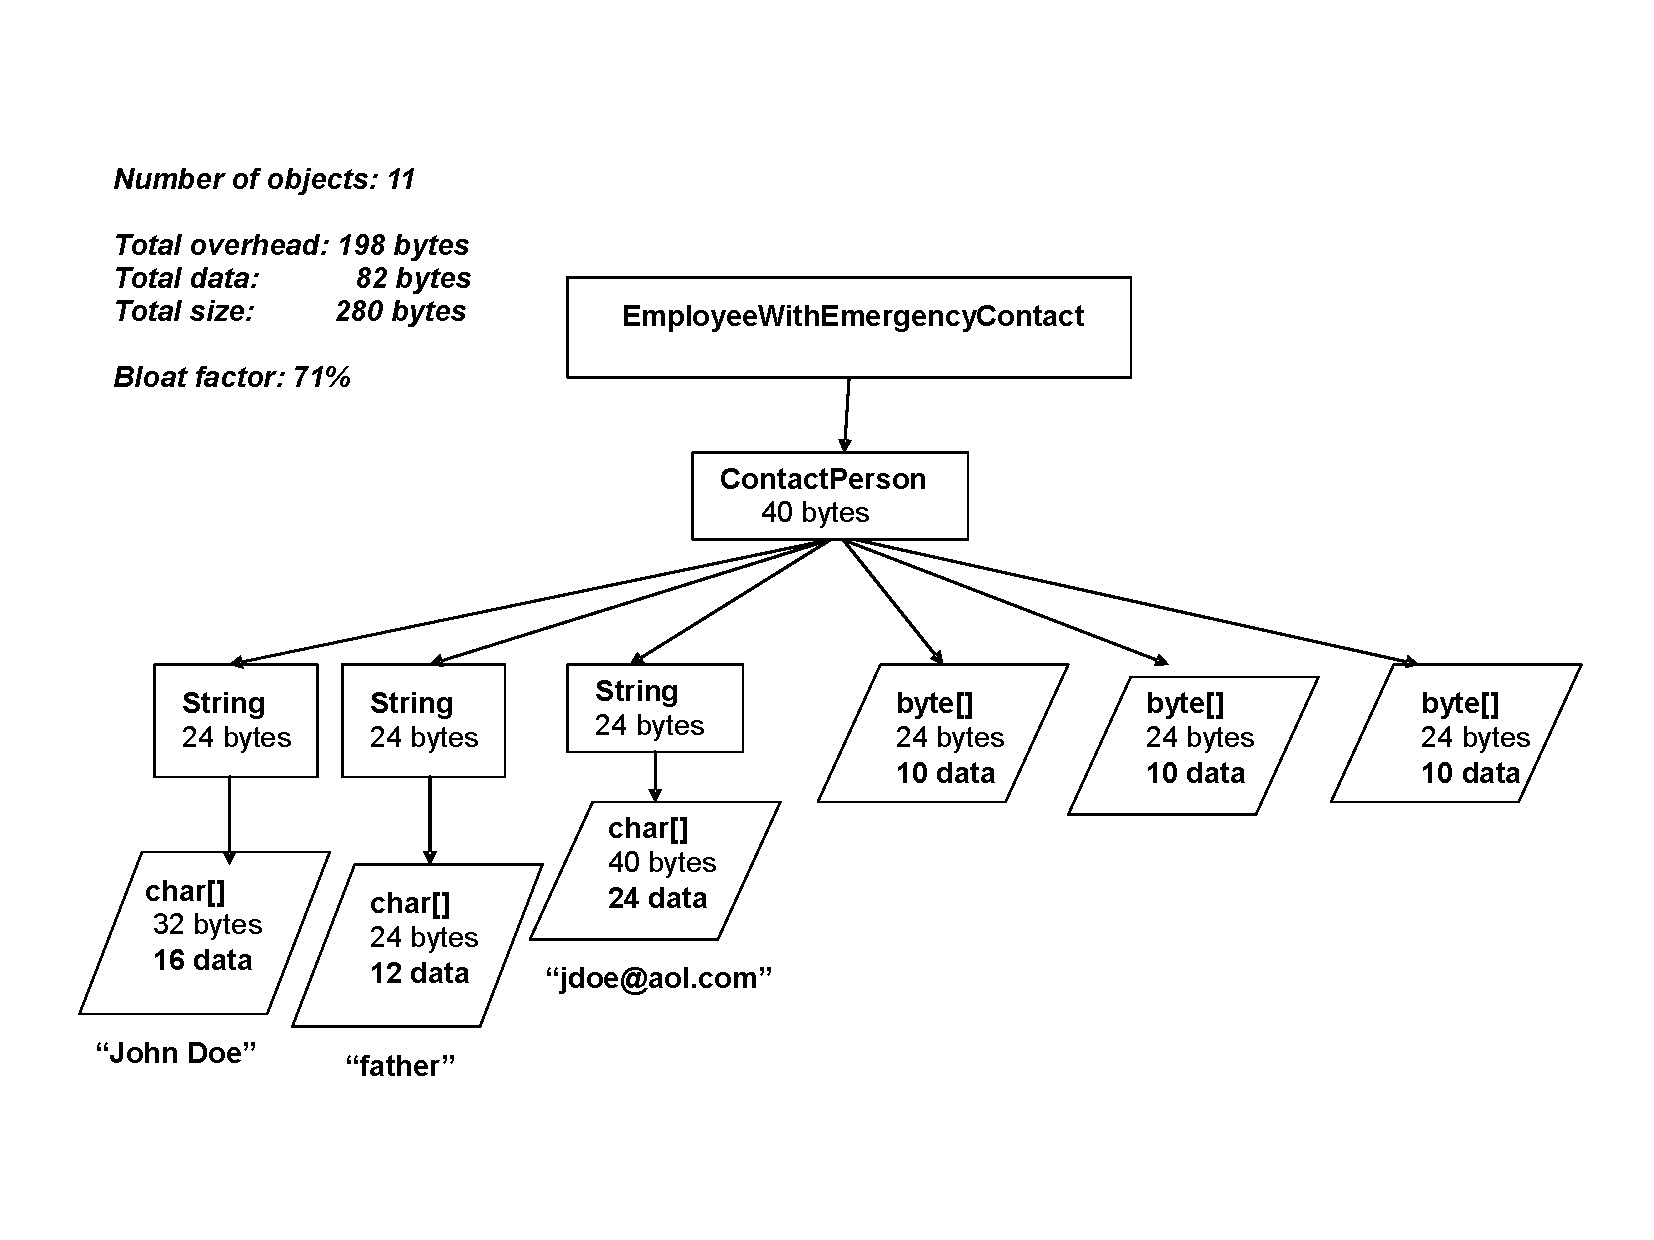
\includegraphics[width=\textwidth]{part1/Figures/modelingdatatypes/refactored-fine-grain.pdf}
 % 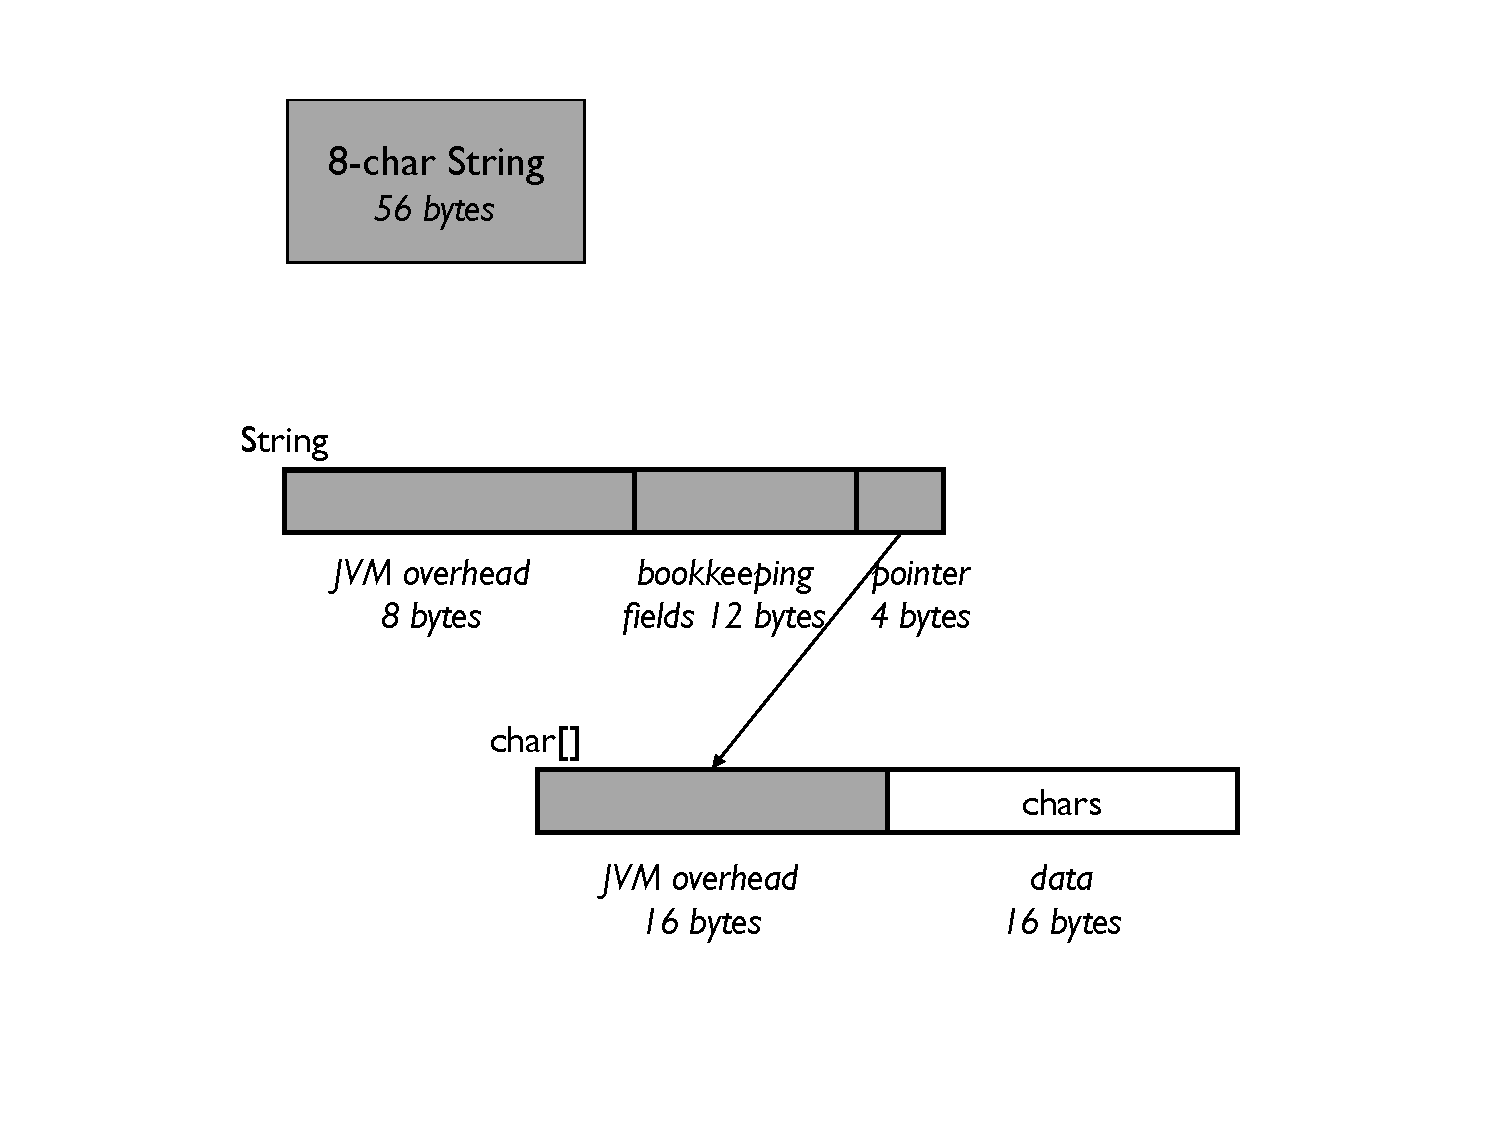
\includegraphics{eight-char-string}
  \caption{The memory layout for an emergency contact, with a more streamlined
  design.}
  \label{fig:refactored-fine-grain}
\end{figure}

When many objects are used to represent one logical concept, this is an indication that the
data model may be using too much delegation. Delegation is good, but it is possible to overuse a good thing.
A design with fewer, bigger objects has less overhead and is more scalable. Whenever you use delegation, there should
be a good reason. This is especially true for the important data entities in an application, those that will determine
the scalability of the program.  
 
 
\section{64-bit Architectures}
\index{64-bit}

If your application does not fit into memory, perhaps moving to a 64-bit architecture will save you. 
However, to support a 64-bit address space, more memory is required. Object header sizes double, and pointers are
8 bytes instead of 4. Some studies~\cite{compressedAddress} show that memory consumption can increase by 40\%-50\%
going from a 32-bit to a 64-bit address space for the same Java program.

%\begin{example}{8-character string} 
Consider what happens to the 8-character string from
Section~\ref{sec:bloat-def} in a 64-bit \jre. The memory layout is shown in
Figure~\ref{fig:8-char-string-64-bit}. The 64-bit string is 43\% bigger than the
32-bit string. All of the additional cost is overhead. Fine-grained designs
and those with a lot of pointers will suffer the most when moving to 64-bit
architectures.
%\end{example}
 
 \begin{figure}
  \centering

 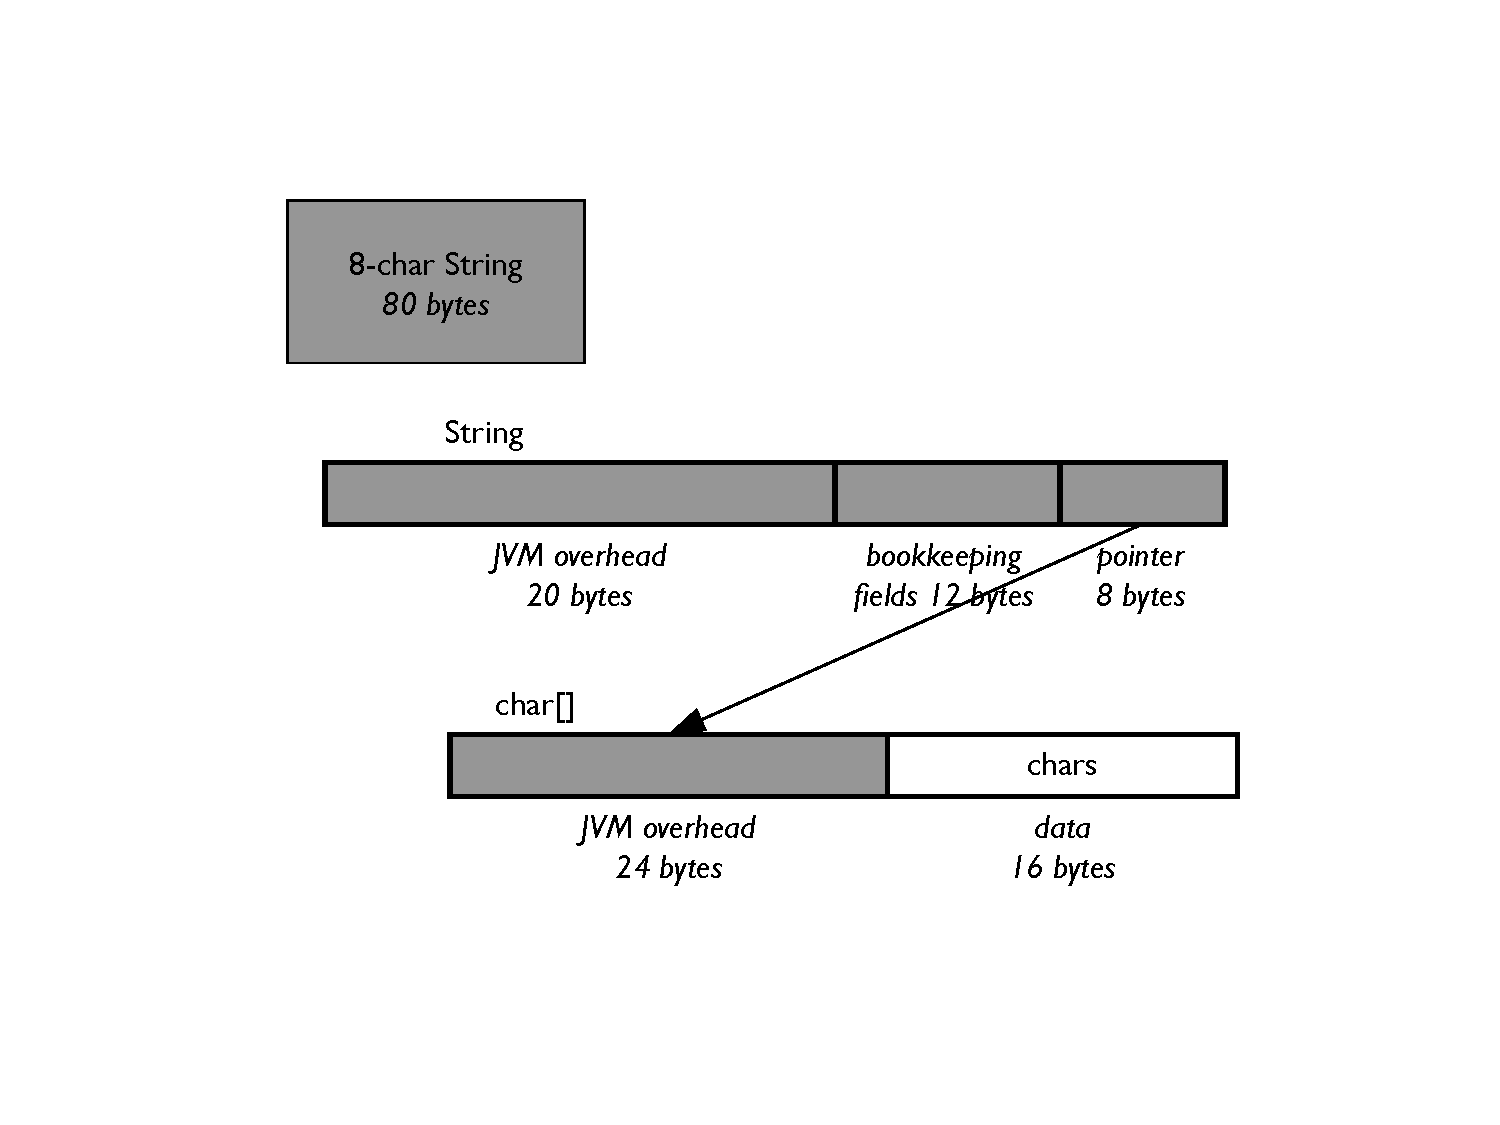
\includegraphics[width=0.8\textwidth]{part1/Figures/modelingdatatypes/8-char-string-64-bit.pdf}
 % 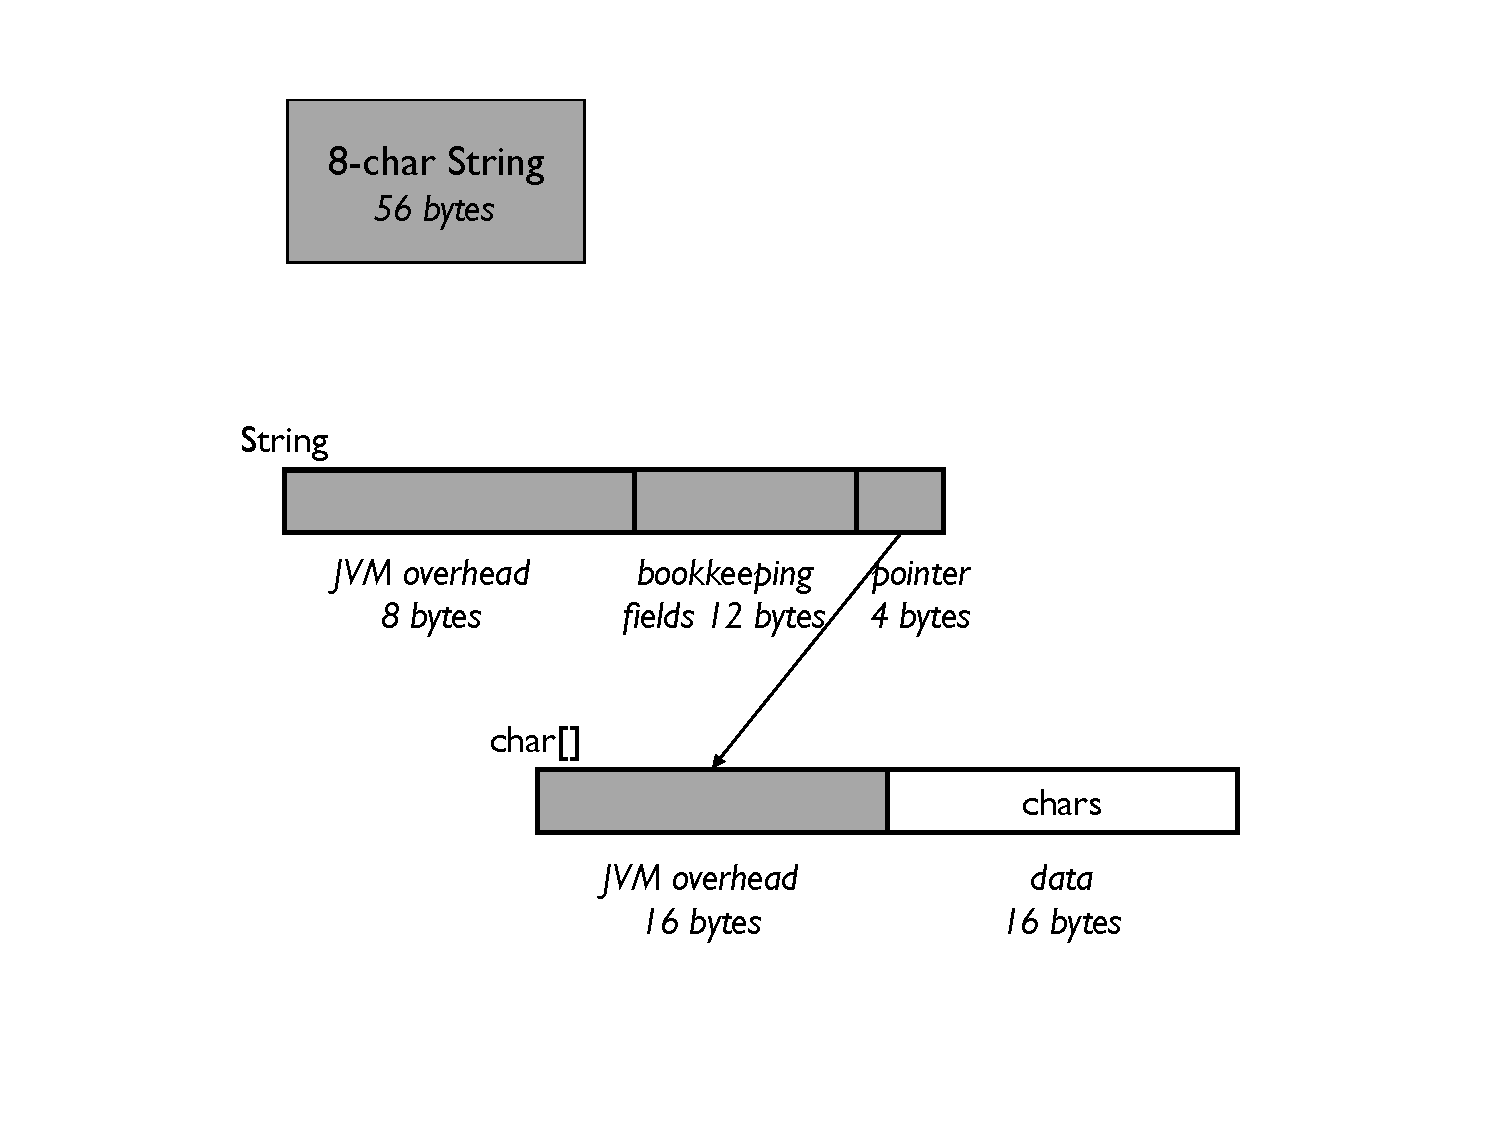
\includegraphics{eight-char-string}
  \caption{The memory layout for an 8-character string on a 64-bit \jre.}
  \label{fig:8-char-string-64-bit}
\end{figure}

Fortunately, in practice things are not always so bad. Both the \oracle and the
\ibm \jres have implemented a scheme for compressing addresses that avoids this blowup, provided that the heap is
less than 32 gigabytes. Address compression is implemented by stealing a few unused bits from 32-bit pointers.
Objects are laid out just like in a 32-bit
address space. During execution, 32-bit compressed addresses are converted into
64-bit native addresses, and vice-versa.  See Appendix~\ref{chapter:jre-comparison} for the
specifics of using this feature.


\section{Summary}

The decisions you make about the \emph{granularity} of your design --- the
number of objects you use to model each record --- will have a big impact on
the memory needs of your system. 
Software engineering best practices and Java's design
both encourage having many small objects.
Since each object comes with memory overhead, it's easy to
produce a data model with a high bloat factor. Estimating your
memory costs will let you weigh the importance of
flexibility and other software engineering goals as you map your data into classes. To estimate the size of
your data, consider:
\begin{itemize}
  \item  The size of each object is the sum of the object header and the field
  sizes, rounded up to an alignment boundary. Header size, alignment, and field
  packing rules all depend on the \jre (see \autoref{chapter:jre-comparison}).
  \item Each time fields are \emph{delegated} to a separate object,
  a new object header and possibly an alignment overhead are introduced, plus
  space for a pointer. While one level of indirection may not seem like much,
  these overheads add up quickly in a fine-grained
  design with many small objects. This is a common reason for memory bloat in
  many applications.
  \item Field types that require one or more separate objects, like
  \class{String}, \class{Date} and \class{BigDecimal}, can add a lot of
  overhead.
  To estimate the cost of a data type, include all of the objects directly
  or indirectly hanging off of it.
  \item Memory overhead will be \emph{much higher} when you switch to a 64-bit
  architecture, unless you can take advantage of compressed addressing. 
  That's especially true for fine-grained designs.
\end{itemize}

Java gives you few modeling options compared to a language
like C++, as shown in \autoref{tab:java-modeling-features}. You are often forced to create
extra objects to solve a design problem, making your alternatives expensive.
The next two chapters guide you through the cost tradeoffs of the most common
patterns when designing data types.

\begin{table}[h]
  \centering
\begin{tabular}{lcc} \toprule
	Feature & Java & C++ \\ \midrule
	Point from one class or array to another & yes & yes \\
	Embed one class or array within another & & yes \\
	Single inheritance & yes & yes \\
	Multiple inheritance &  & yes \\
	Union types & & yes \\
	\bottomrule
\end{tabular}
 % 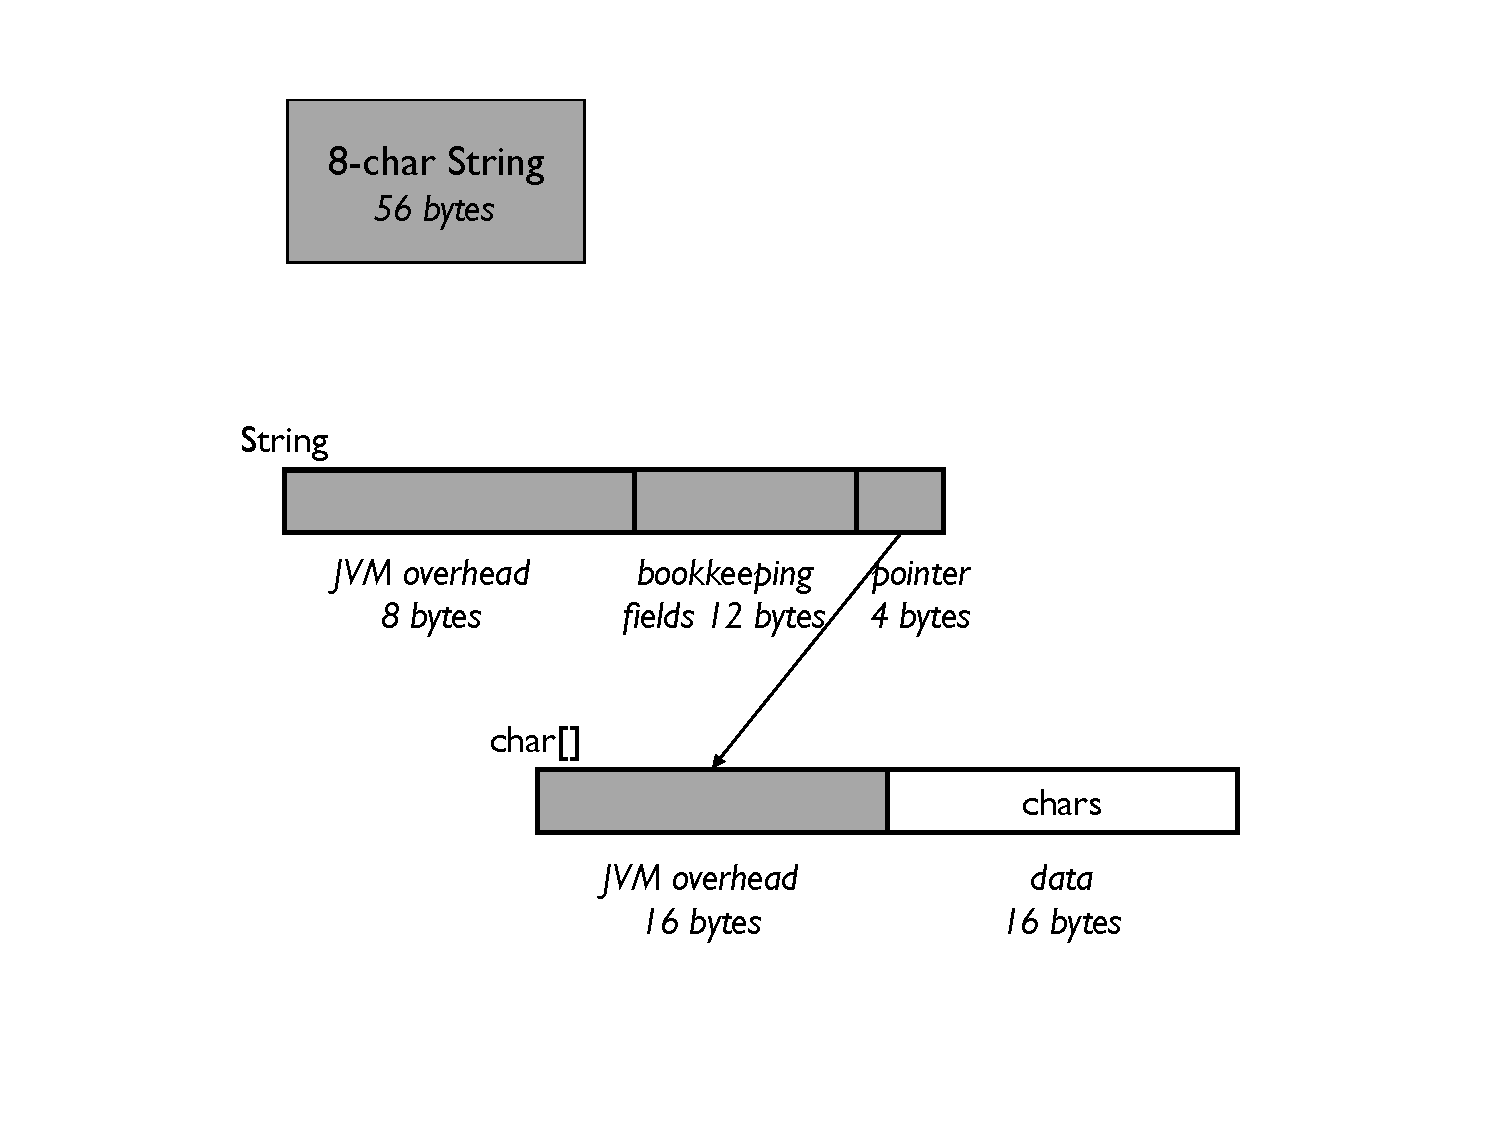
\includegraphics{eight-char-string}
  \caption{Java's simpler approach to modeling means designs rely heavily on
  delegation.}
  \label{tab:java-modeling-features}
  \index{Modeling Comparison C++}
\end{table}


